\documentclass[UTF8,fontset=none,zihao=-4,a4paper]{ctexart}
\usepackage[left=26mm,right=26mm,top=25mm,bottom=25mm,headheight=15pt]{geometry}
\setCJKmainfont{Songti SC}[BoldFont={Songti SC Bold}]
\setCJKsansfont{Songti SC}[BoldFont={Songti SC Bold}]
\setCJKmonofont{Songti SC}[BoldFont={Songti SC Bold}]
\setmainfont{Times New Roman}
\usepackage{amsmath,amssymb,booktabs,tabularx,array,enumitem,fancyhdr,needspace,longtable,tikz}
\usetikzlibrary{arrows.meta}
\usepackage[hidelinks]{hyperref}
\hypersetup{pdftitle={离散数学},pdfsubject={命题逻辑、一阶逻辑、集合代数与二元关系讲义}}
\ctexset{section={format=\large\bfseries,beforeskip=0pt,afterskip=14pt},subsection={format=\normalsize\bfseries,beforeskip=12pt,afterskip=6pt}}
\setcounter{tocdepth}{1}
\linespread{1.22}
\setlength{\parindent}{2em}
\setlength{\parskip}{3pt}
\setlength{\tabcolsep}{6pt}
\renewcommand{\arraystretch}{1.35}
\setlist{itemsep=4pt,topsep=5pt,parsep=0pt,leftmargin=2em}
\setlist[enumerate]{label=\arabic*.}
\pagestyle{fancy}
\fancyhf{}
\fancyhead[L]{\small 离散数学}
\fancyhead[R]{\small\nouppercase{\leftmark}}
\fancyfoot[C]{\small\thepage}
\renewcommand{\headrulewidth}{0.3pt}
\renewcommand{\sectionmark}[1]{\markboth{#1}{}}
\newcommand{\chapterpage}[1]{\clearpage\section{#1}}
\newcommand{\example}[1]{\par\Needspace{5\baselineskip}\noindent\textbf{例：#1}\par}
\newcommand{\note}[1]{\par\noindent\textbf{说明：}#1\par}
\newcommand{\exercise}{\subsection{本章练习与参考解答}}
\newcommand{\term}[1]{\textbf{#1}}
\newcolumntype{Y}{>{\raggedright\arraybackslash}X}
\allowdisplaybreaks[2]
\raggedbottom
\begin{document}
\begin{titlepage}
\thispagestyle{empty}
\vspace*{0.28\textheight}
\begin{center}
{\fontsize{36}{45}\selectfont\bfseries 离散数学}
\end{center}
\end{titlepage}
\pagenumbering{Roman}
\thispagestyle{empty}
\tableofcontents
\clearpage
\pagenumbering{arabic}

\section{命题逻辑基本概念}
命题逻辑研究陈述的真值及其联结结构。本章依次讨论命题的识别、联结词、自然语言的符号化、合式公式、赋值与真值表。真值统一用 $1$ 和 $0$ 表示。

\subsection{命题、真值与命题分类}
\term{命题}是具有确定真值的陈述句。真值为 $1$ 的称为真命题，为 $0$ 的称为假命题。判断结果唯一确定，不等于目前已经知道判断结果。指定时间、地点的未来事件可以构成命题；真值暂时未知不影响其命题身份。

\term{简单命题}（原子命题）不能再分解为由联结词连接的命题；\term{复合命题}由简单命题和联结词构成。分类依据逻辑结构，而非句子长短或是否出现“和”“与”等字。
\example{识别命题与原子结构}
“$2+5=7$”是真命题；“$2$ 是合数”是假命题；“$x+5>3$”在 $x$ 未指定且未量化时是含变量的开语句；疑问句、祈使句、感叹句和无法一致确定真值的悖论不作为本课程的命题。
“张辉与王丽都是三好学生”可分成两个命题的合取；“张辉与王丽是同学”描述一个关系，在命题逻辑中作为一个简单命题。“豆沙包由面粉和红小豆做成”中的“和”连接原料名称，不能据此拆成两个命题。

一个具体命题具有固定真值，可称为\term{命题常项}；命题变项（命题变元）是代表任意命题真值的符号，通常记为 $p,q,r,\ldots$。应区分具体陈述、表示陈述的符号和符号的赋值。

\subsection{五种基本联结词}
\begin{center}
\begin{tabularx}{\linewidth}{l c Y}
\toprule 名称 & 公式 & 真值条件\\\midrule
否定 & $\neg p$ & $p$ 假时真，$p$ 真时假\\
合取 & $p\land q$ & $p,q$ 同时为真时真\\
析取 & $p\lor q$ & $p,q$ 至少一个为真时真\\
蕴涵 & $p\to q$ & 仅当前件 $p$ 真、后件 $q$ 假时假\\
等价（双条件） & $p\leftrightarrow q$ & $p,q$ 真值相同时真\\\bottomrule
\end{tabularx}
\end{center}
\begin{center}
\begin{tabular}{cc|ccccc}
\toprule $p$&$q$&$\neg p$&$p\land q$&$p\lor q$&$p\to q$&$p\leftrightarrow q$\\\midrule
0&0&1&0&0&1&1\\
0&1&1&0&1&1&0\\
1&0&0&0&1&0&0\\
1&1&0&1&1&1&1\\\bottomrule
\end{tabular}
\end{center}
“虽然 $p$，但是 $q$”“不仅 $p$，而且 $q$”均按 $p\land q$ 处理；联结词只记录真值关系，不记录转折、强调或因果的修辞信息。

析取 $p\lor q$ 默认是\term{相容或}，允许二者同真。\term{排斥或}要求恰好一个为真，记作 $p\oplus q$，其基本表达式为
\[
p\oplus q\equiv(p\land\neg q)\lor(\neg p\land q)
\equiv(p\lor q)\land\neg(p\land q).
\]
“至少一人参加”用析取；“一人且仅一人参加”用排斥或。若实际背景已保证二者不能同真，可以另行说明背景约束，不能把普通析取本身解释为排斥或。

\subsection{充分条件、必要条件与蕴涵符号化}
$p\to q$ 表示 $p$ 是 $q$ 的充分条件，$q$ 是 $p$ 的必要条件。当 $p$ 为假时，蕴涵式恒真，称为空真；这不表示后件实际为真。
\begin{center}
\begin{tabularx}{\linewidth}{Y c}
\toprule 自然语言 & 形式\\\midrule
如果 $p$，则 $q$；只要 $p$，就 $q$ & $p\to q$\\
$p$ 仅当 $q$；只有 $q$，才 $p$ & $p\to q$\\
除非 $q$，否则非 $p$；$p$ 只有在 $q$ 时才发生 & $p\to q$\\
除非 $p$，否则 $q$ & $\neg p\to q$\\
$p$ 当且仅当 $q$；$p,q$ 互为充要条件 & $p\leftrightarrow q$\\\bottomrule
\end{tabularx}
\end{center}
\example{天冷与穿羽绒服}
设 $p$：天冷，$q$：小王穿羽绒服。
“只要天冷，就穿羽绒服”为 $p\to q$；“只有天冷，才穿羽绒服”为 $q\to p$；“不穿羽绒服，则天不冷”为 $\neg q\to\neg p$；“除非穿羽绒服，否则天不冷”为 $\neg q\to\neg p$。
\[
p\to q\equiv\neg q\to\neg p.
\]
原命题 $p\to q$ 的\term{逆命题}是 $q\to p$，\term{否命题}是 $\neg p\to\neg q$，\term{逆否命题}是 $\neg q\to\neg p$。原命题与逆否命题等值，逆命题与否命题等值，两组之间一般不等值。

\subsection{合式公式、子公式与层次}
\term{合式公式}的递归定义为：原子命题公式是公式；若 $A$ 是公式，则 $(\neg A)$ 是公式；若 $A,B$ 是公式，则 $(A\land B)$、$(A\lor B)$、$(A\to B)$、$(A\leftrightarrow B)$ 是公式；只有有限次应用上述规则得到的符号串才是公式。

构造公式时使用的较小公式称为\term{子公式}。最外层的联结词是主联结词。课件采用的优先顺序是
\[
\neg\quad>\quad\land\quad>\quad\lor\quad>\quad\to\quad>\quad\leftrightarrow.
\]
括号优先，先内后外；课件约定同级从左到右。蕴涵没有结合律，连续蕴涵宜写全括号以明确结构。

令 $h(A)$ 为公式层次：原子公式 $h(p)=0$；$h(\neg A)=h(A)+1$；对二元联结词 $\circ$，
\[
h(A\circ B)=1+\max\{h(A),h(B)\}.
\]
层次衡量嵌套深度，不是联结词总数。例如 $\neg p\to q$ 为 $2$ 层，$\neg(p\to q)\leftrightarrow r$ 为 $3$ 层，
$((\neg p\land q)\to r)\leftrightarrow(\neg r\lor s)$ 为 $4$ 层。

\subsection{赋值、真值表与公式类型}
对公式中每个命题变元指定一个真值，称为一个\term{赋值}或解释。含 $n$ 个不同变元的公式共有 $2^n$ 个赋值。固定变元顺序 $p,q,r$ 后，字符串 $101$ 表示 $p=1,q=0,r=1$。使公式为真的赋值称为成真赋值，使公式为假的称为成假赋值。

\term{真值表}列出公式在全部赋值下的真值。构造步骤为：确定不同变元及顺序；按二进制从 $00\cdots0$ 排到 $11\cdots1$；按子公式由内向外逐列计算；据最后一列汇总赋值与类型。
\example{完整真值表}
设 $F=(p\lor q)\to\neg r$。
\begin{center}
\begin{tabular}{ccc|ccc}
\toprule $p$&$q$&$r$&$p\lor q$&$\neg r$&$F$\\\midrule
0&0&0&0&1&1\\
0&0&1&0&0&1\\
0&1&0&1&1&1\\
0&1&1&1&0&0\\
1&0&0&1&1&1\\
1&0&1&1&0&0\\
1&1&0&1&1&1\\
1&1&1&1&0&0\\\bottomrule
\end{tabular}
\end{center}
成真赋值为 $000,001,010,100,110$；成假赋值为 $011,101,111$。

\term{重言式}（永真式）在每个赋值下为真；\term{矛盾式}（永假式）在每个赋值下为假；\term{可满足式}至少有一个成真赋值。重言式是可满足式，逆向不成立。既有成真赋值又有成假赋值的公式称为非重言式的可满足式，也称偶然式。
\[
p\lor\neg p\text{ 是重言式},\qquad
p\land\neg p\text{ 是矛盾式}.
\]
设 $T(F)$ 为成真赋值集合，则重言式对应全部赋值，矛盾式对应空集，偶然式对应非空真子集。$F$ 永真当且仅当 $\neg F$ 不可满足；$F$ 可满足当且仅当 $\neg F$ 非永真。

\exercise
\begin{enumerate}
\begin{samepage}
\item 设 $p$：交通阻塞，$q$：某人迟到。将“交通不阻塞就不迟到”“没迟到，所以交通没阻塞”“迟到仅当交通阻塞”符号化。\\
\term{解：}$\neg p\to\neg q$、$\neg q\to\neg p$、$q\to p$。第一式与第三式等值；第二式与 $p\to q$ 等值。
\end{samepage}
\begin{samepage}
\item 求 $\neg(p\to q)\land q$ 的类型。\\
\term{解：}$p\to q$ 假要求 $p=1,q=0$，但合取又要求 $q=1$，故无成真赋值，是矛盾式。
\end{samepage}
\begin{samepage}
\item 判断 $(p\to q)\leftrightarrow(p\to r)$ 的类型，并列出成假赋值。\\
\term{解：}$p=0$ 时两侧均真；$p=1$ 时比较 $q,r$。仅 $101,110$ 使公式为假，故为非重言式的可满足式。
\end{samepage}
\begin{samepage}
\item 求 $\neg((p\lor q)\to r)$ 的层次及成真赋值。\\
\term{解：}层次为 $3$；要求 $p\lor q=1,r=0$，成真赋值为 $010,100,110$。
\end{samepage}
\end{enumerate}
\note{识别命题时不以“现在能否求出真值”为标准；符号化时先确定原子陈述，再辨析“或”和条件方向；真值表必须列出全部不同变元，不能只列部分组合。}

\chapterpage{命题逻辑等值演算}
\subsection{等值式与记号的层次}
若 $A\leftrightarrow B$ 为重言式，则称 $A,B$ 逻辑等值，记为 $A\equiv B$。课件用 $A\Leftrightarrow B$ 表示同一关系。$\leftrightarrow$ 是公式内部的双条件联结词；$\equiv$ 是公式之间的关系，不是另一种命题联结词。

等值具有自反性、对称性、传递性。比较两个公式时，应在它们所含变元的并集上赋值。某变元虽在公式表面出现，却不影响真值，称为真值函数意义下的哑元。例如 $p\lor(r\land\neg r)\equiv p$ 中 $r$ 不影响输出；这与一阶逻辑中约束变量的称谓应结合上下文区分。

\subsection{十六组基本等值式}
下表中的 $A,B,C$ 可为任意公式，$1,0$ 分别代表真、假。
\begingroup
\renewcommand{\arraystretch}{1.12}
\begin{longtable}{p{0.18\linewidth}p{0.75\linewidth}}
\toprule 名称 & 等值式\\\midrule\endhead
双重否定律 & $\neg\neg A\equiv A$\\
幂等律 & $A\lor A\equiv A$；$A\land A\equiv A$\\
交换律 & $A\lor B\equiv B\lor A$；$A\land B\equiv B\land A$\\
结合律 & $(A\lor B)\lor C\equiv A\lor(B\lor C)$；\newline $(A\land B)\land C\equiv A\land(B\land C)$\\
分配律 & $A\lor(B\land C)\equiv(A\lor B)\land(A\lor C)$；\newline $A\land(B\lor C)\equiv(A\land B)\lor(A\land C)$\\
德摩根律 & $\neg(A\lor B)\equiv\neg A\land\neg B$；\newline $\neg(A\land B)\equiv\neg A\lor\neg B$\\
吸收律 & $A\lor(A\land B)\equiv A$；$A\land(A\lor B)\equiv A$\\
零律 & $A\lor1\equiv1$；$A\land0\equiv0$\\
同一律 & $A\lor0\equiv A$；$A\land1\equiv A$\\
排中律 & $A\lor\neg A\equiv1$\\
矛盾律 & $A\land\neg A\equiv0$\\
蕴涵等值式 & $A\to B\equiv\neg A\lor B$\\
等价等值式 & $A\leftrightarrow B\equiv(A\to B)\land(B\to A)$\\
假言易位 & $A\to B\equiv\neg B\to\neg A$\\
等价否定式 & $A\leftrightarrow B\equiv\neg A\leftrightarrow\neg B$\\
归谬论 & $(A\to B)\land(A\to\neg B)\equiv\neg A$\\\bottomrule
\end{longtable}
\endgroup
还常用双条件的析取表达式：
\[
A\leftrightarrow B\equiv(A\land B)\lor(\neg A\land\neg B).
\]

\subsection{置换规则与等值演算}
若 $A\equiv B$，可在公式 $\Phi(A)$ 中将指定的子公式 $A$ 换为 $B$，得到等值公式 $\Phi(B)$。这称为\term{置换规则}。把基本等值式中的命题变元一致代入公式，是产生等值式实例；对既有公式的子公式进行等值置换，是利用实例完成变形。

\example{嵌套蕴涵的等值证明}
\begin{align*}
p\to(q\to r)
&\equiv\neg p\lor(\neg q\lor r) &&\text{蕴涵等值式}\\
&\equiv(\neg p\lor\neg q)\lor r &&\text{结合律}\\
&\equiv\neg(p\land q)\lor r &&\text{德摩根律}\\
&\equiv(p\land q)\to r &&\text{蕴涵等值式}.
\end{align*}
但 $(p\to q)\to r$ 与 $p\to(q\to r)$ 不等值：赋值 $000$ 使前者为 $0$、后者为 $1$。证明不等值，只需给出一个真值不同的赋值；化简后的外观不同不构成充分证据。

\example{化简与类型判定}
\begin{align*}
q\land\neg(p\to q)&\equiv q\land p\land\neg q\equiv0,\\
(p\to q)\leftrightarrow(\neg q\to\neg p)&\equiv1,\\
((p\land q)\lor(p\land\neg q))\land r
&\equiv p\land(q\lor\neg q)\land r\equiv p\land r.
\end{align*}
三式分别为矛盾式、重言式、非重言式的可满足式。等值演算中的每一步应注明或能明确识别依据的算律。

\subsection{文字、简单式与普通范式}
\term{文字}是命题变元或其否定。\term{简单合取式}是有限个文字的合取；\term{简单析取式}是有限个文字的析取。\term{析取范式}（DNF）是若干简单合取式的析取；\term{合取范式}（CNF）是若干简单析取式的合取。单个文字既是简单合取式，也是简单析取式；一个简单式也可同时看成两类范式。
\[
(p\land\neg q)\lor(q\land r)\text{ 为 DNF},\qquad
(p\lor q)\land(\neg p\lor r)\text{ 为 CNF}.
\]
简单析取式是重言式，当且仅当它同时含有某变元及其否定；简单合取式是矛盾式，当且仅当它同时含有某变元及其否定。DNF 是矛盾式，当且仅当每个合取项都矛盾；CNF 是重言式，当且仅当每个析取子句都永真。不能交换上述判定方向，例如 $p\lor\neg p$ 的两个 DNF 合取项分别都不是重言式，但整体是重言式。

\term{范式存在定理：}每个命题公式都存在等值的 DNF 和 CNF，普通范式不唯一。转换步骤为：消去 $\to,\leftrightarrow$；将否定移到变元之前；采用合适方向的分配律；用幂等、吸收及矛盾律整理。
\example{求两类范式}
\begin{align*}
(p\to\neg q)\to r
&\equiv\neg(\neg p\lor\neg q)\lor r\\
&\equiv(p\land q)\lor r &&\text{DNF}\\
&\equiv(p\lor r)\land(q\lor r) &&\text{CNF}.
\end{align*}
注意求 DNF 用 $\land$ 对 $\lor$ 的分配，求 CNF 用 $\lor$ 对 $\land$ 的分配，不能仅凭最终出现哪个联结词判断。

\subsection{极小项、极大项及二进制编号}
固定 $n$ 个变元及顺序后，每个变元恰好出现一次、正负形式择一的简单合取式称为\term{极小项}（最小项）；相应的简单析取式称为\term{极大项}（最大项）。各有 $2^n$ 个。

$m_i$ 仅在编号 $i$ 的赋值为真：二进制位为 $1$ 取正文字，为 $0$ 取负文字。$M_i$ 仅在编号 $i$ 的赋值为假：二进制位为 $0$ 取正文字，为 $1$ 取负文字。因此 $\neg m_i\equiv M_i$，$\neg M_i\equiv m_i$。
\begin{center}
\begin{tabular}{c c l l}
\toprule 编号 & $pqr$ & $m_i$ & $M_i$\\\midrule
0&000&$\neg p\land\neg q\land\neg r$&$p\lor q\lor r$\\
1&001&$\neg p\land\neg q\land r$&$p\lor q\lor\neg r$\\
2&010&$\neg p\land q\land\neg r$&$p\lor\neg q\lor r$\\
3&011&$\neg p\land q\land r$&$p\lor\neg q\lor\neg r$\\
4&100&$p\land\neg q\land\neg r$&$\neg p\lor q\lor r$\\
5&101&$p\land\neg q\land r$&$\neg p\lor q\lor\neg r$\\
6&110&$p\land q\land\neg r$&$\neg p\lor\neg q\lor r$\\
7&111&$p\land q\land r$&$\neg p\lor\neg q\lor\neg r$\\\bottomrule
\end{tabular}
\end{center}
不同极小项互斥：$m_i\land m_j\equiv0$（$i\ne j$）；所有极小项的析取为 $1$。不同极大项的析取为 $1$，所有极大项的合取为 $0$。

\subsection{主范式的存在、唯一性与求法}
\term{主析取范式}（PDNF）由极小项组成，\term{主合取范式}（PCNF）由极大项组成。固定变元全集和顺序后，它们唯一，忽略项的排列和重复。若改变变元全集或顺序，编号表示也会改变。

主析取范式取所有成真行对应的极小项，主合取范式取所有成假行对应的极大项。设 $U=\{0,\ldots,2^n-1\}$，成真编号集为 $S$，则
\[
F\equiv\bigvee_{i\in S}m_i\equiv\bigwedge_{i\in U\setminus S}M_i.
\]
也记为 $\Sigma m(S)$ 与 $\Pi M(U\setminus S)$。空析取约定为 $0$，空合取约定为 $1$，从而涵盖矛盾式和重言式。

等值演算求主析取范式时，先求 DNF，去掉矛盾项和重复文字，再给缺少 $p$ 的合取项 $B$ 补入
\[
B\equiv B\land(p\lor\neg p)\equiv(B\land p)\lor(B\land\neg p).
\]
求主合取范式时，先求 CNF，删去永真子句，对缺少 $p$ 的子句 $C$ 使用
\[
C\equiv C\lor(p\land\neg p)\equiv(C\lor p)\land(C\lor\neg p).
\]
最后消除重复项，按编号排序。也可直接由真值表求主范式。
\example{课件中的三变元主范式}
对 $F=(p\to\neg q)\to r\equiv(p\land q)\lor r$，
\[
p\land q\equiv m_6\lor m_7,\qquad
r\equiv m_1\lor m_3\lor m_5\lor m_7.
\]
故
\[
F\equiv\Sigma m(1,3,5,6,7)\equiv\Pi M(0,2,4).
\]
成真赋值为 $001,011,101,110,111$；成假赋值为 $000,010,100$。

\subsection{主范式的应用与逻辑建模}
若 PDNF 含 $s$ 个不同极小项，则有 $s$ 个成真赋值和 $2^n-s$ 个成假赋值。$s=2^n$ 时重言，$s=0$ 时矛盾，其余情况为偶然式。在相同变元全集和顺序下，两个公式等值，当且仅当其成真编号集合相同。

\example{三人选派问题}
设 $p,q,r$ 分别表示选派 $A,B,C$。约束为：$A$ 去则 $C$ 去；$B$ 去则 $C$ 不去；$A,B$ 恰好一人去。
\begin{align*}
F&=(p\to r)\land(q\to\neg r)\land(p\oplus q)\\
&\equiv(p\land\neg q\land r)\lor(\neg p\land q\land\neg r)\\
&\equiv m_5\lor m_2.
\end{align*}
两种方案分别为选派 $A,C$，或仅选派 $B$。各项约束应合取，不能析取。

\example{五人选派问题}
设 $p,q,r,s,u$ 分别表示赵、钱、孙、李、周被选派。条件是赵去则钱去，李周至少一人去，钱孙恰好一人去，孙李同去或同不去，周去则赵钱都去：
\[
F=(p\to q)\land(s\lor u)\land(q\oplus r)
\land(r\leftrightarrow s)\land(u\to(p\land q)).
\]
若 $r=1$，则 $q=0,s=1,p=0,u=0$；若 $r=0$，则 $q=1,s=0,u=1,p=1$。故全部成真赋值为 $00110,11001$，即选派孙、李，或选派赵、钱、周。

\subsection{真值函数与联结词完备集}
\term{$n$ 元真值函数}是映射 $F:\{0,1\}^n\to\{0,1\}$。输入有 $2^n$ 种，每个输入可独立指定输出，故真值函数总数为 $2^{2^n}$：一元有 $4$ 个，二元有 $16$ 个，三元有 $256$ 个。每个命题公式决定一个真值函数；多个等值公式决定同一个函数。

若任何 $n\ge1$ 元真值函数都可由只含集合 $S$ 中联结词的公式表示，则 $S$ 是\term{联结词完备集}。由范式存在定理，$\{\neg,\land,\lor\}$ 完备。以下也都完备：
\[
\{\neg,\land\},\quad\{\neg,\lor\},\quad\{\neg,\to\}.
\]
理由是 $A\lor B\equiv\neg(\neg A\land\neg B)$、$A\land B\equiv\neg(\neg A\lor\neg B)$、$A\lor B\equiv\neg A\to B$。完备集的任何超集仍完备。

当不额外提供常值 $0$ 时，$\{\land,\lor,\to,\leftrightarrow\}$ 不完备：全部输入为 $1$ 时，只用这些联结词构造的公式恒输出 $1$，不能表示否定或恒假函数。证明不完备可寻找整个集合保持而目标函数不保持的性质。

定义\term{与非} $p\uparrow q\equiv\neg(p\land q)$、\term{或非} $p\downarrow q\equiv\neg(p\lor q)$，二者单独均构成完备集：
\begin{align*}
\neg p&\equiv p\uparrow p, & \neg p&\equiv p\downarrow p,\\
p\land q&\equiv(p\uparrow q)\uparrow(p\uparrow q),
& p\land q&\equiv(p\downarrow p)\downarrow(q\downarrow q),\\
p\lor q&\equiv(p\uparrow p)\uparrow(q\uparrow q),
& p\lor q&\equiv(p\downarrow q)\downarrow(p\downarrow q).
\end{align*}
\example{用指定联结词改写}
令 $A=(p\to\neg q)\land r$。
\begin{align*}
A&\equiv\neg(p\land q)\land r &&\{\neg,\land\},\\
A&\equiv\neg(\neg(\neg p\lor\neg q)\lor\neg r) &&\{\neg,\lor\},\\
A&\equiv\neg((p\to\neg q)\to\neg r) &&\{\neg,\to\},\\
A&\equiv((p\uparrow q)\uparrow r)\uparrow((p\uparrow q)\uparrow r) &&\{\uparrow\},\\
A&\equiv((p\downarrow p)\downarrow(q\downarrow q))\downarrow(r\downarrow r)
&&\{\downarrow\}.
\end{align*}

\exercise
\begin{enumerate}
\begin{samepage}
\item 按 $p,q,r$ 顺序，已知 $F$ 的成真赋值为 $001,010,111$，求两类主范式。\\
\term{解：}$F\equiv\Sigma m(1,2,7)\equiv\Pi M(0,3,4,5,6)$。
\end{samepage}
\begin{samepage}
\item 设 $F\equiv\Sigma m(1,2,4)$，求 $\neg F$ 的 PDNF 与 $F$ 的 PCNF（共三变元）。\\
\term{解：}两者的编号都是 $0,3,5,6,7$，但前者使用 $m_i$，后者使用 $M_i$。
\end{samepage}
\begin{samepage}
\item 求 $(p\to q)\land\neg p$ 的主范式。\\
\term{解：}公式等值于 $\neg p$，故为 $m_0\lor m_1$，也为 $M_2\land M_3$。
\end{samepage}
\begin{samepage}
\item 判断“每个 CNF 都可满足”。\\
\term{解：}错误，CNF $p\land\neg p$ 不可满足。普通范式的结构并不保证可满足性。
\end{samepage}
\begin{samepage}
\item 只用与非表示 $p\to q$。\\
\term{解：}$p\to q\equiv\neg(p\land\neg q)\equiv p\uparrow(q\uparrow q)$。
\end{samepage}
\end{enumerate}
\chapterpage{命题逻辑的推理理论}
\subsection{推理的形式结构与有效性}
推理由前提 $A_1,\ldots,A_k$ 和结论 $B$ 构成。若每个使全部前提为真的赋值都使 $B$ 为真，则推理有效（正确），记为
\[
\{A_1,\ldots,A_k\}\models B.
\]
课件以重言蕴涵记号 $A_1\land\cdots\land A_k\Rightarrow B$ 表示这一关系。注意 $\to$ 是公式中的蕴涵联结词，$\Rightarrow$ 在此表示该蕴涵式为重言式。
\[
\{A_1,\ldots,A_k\}\models B
\quad\Longleftrightarrow\quad
(A_1\land\cdots\land A_k)\to B\text{ 是重言式}.
\]
等价地，$A_1\land\cdots\land A_k\land\neg B$ 不可满足。反例必须让全部前提同真、结论为假；仅找到结论为假的赋值不足以否定推理。

有效性保证“当前提都真时，结论也真”，并不保证前提在实际世界中为真，也不单独保证结论实际为真。前提互相矛盾时，没有使全部前提为真的赋值，因此在经典逻辑中可语义地蕴涵任意结论。
\example{有效形式与无效形式}
$p\to q,p\models q$ 是假言推理。即使“今天是 $1$ 号则明天是 $5$ 号”在日常意义下为假，该形式仍然有效。
$p\to q,q\not\models p$：$p=0,q=1$ 时两个前提都真而结论假，称为\term{肯定后件错误}。$p\to q,\neg p\not\models\neg q$ 也无效，同一赋值即为反例，称为\term{否定前件错误}。

\subsection{判断推理是否有效的方法}
\begin{enumerate}
\item 真值表法：检查形式结构的蕴涵式是否每行均为 $1$，或只检查全部前提同真的行。
\item 等值演算法：将形式结构化简为 $1$；若不能化为 $1$，仍须进一步判定，不能因化简暂时停止就宣布无效。
\item 主范式法：检验蕴涵式的 PDNF 是否包含全部 $2^n$ 个极小项。
\item 反例法：寻找全部前提同真而结论假的赋值。
\end{enumerate}
\example{错误结论的反例与纠正}
前提为 $\neg p\to q,\neg q$，结论为 $\neg p$。取 $p=1,q=0$，前提都真，结论假，故无效。正确使用拒取式，应由 $\neg p\to q,\neg q$ 得到 $\neg\neg p$，再得到 $p$。

\subsection{推理定律}
以下每个“前提推出结论”的形式均对应重言蕴涵式。$A,B,C,D$ 可代入任意命题公式。
\begin{longtable}{p{0.22\linewidth}p{0.71\linewidth}}
\toprule 名称 & 前提 $\models$ 结论\\\midrule\endhead
附加律 & $A\models A\lor B$\\
化简律 & $A\land B\models A$；$A\land B\models B$\\
假言推理（MP） & $A\to B,\ A\models B$\\
拒取式（MT） & $A\to B,\ \neg B\models\neg A$\\
析取三段论 & $A\lor B,\ \neg B\models A$\\
假言三段论 & $A\to B,\ B\to C\models A\to C$\\
等价三段论 & $A\leftrightarrow B,\ B\leftrightarrow C\models A\leftrightarrow C$\\
构造性二难 & $A\to B,\ C\to D,\ A\lor C\models B\lor D$\\
构造性二难特例 & $A\to B,\ \neg A\to B\models B$\\
破坏性二难 & $A\to B,\ C\to D,\ \neg B\lor\neg D\models\neg A\lor\neg C$\\
合取引入 & $A,\ B\models A\land B$\\\bottomrule
\end{longtable}
每个等值式 $A\equiv B$ 可产生两个推理定律 $A\models B$ 和 $B\models A$。推理定律一般不可逆，例如附加律不能逆向用于从 $A\lor B$ 推出 $A$。
\example{推理定律的语义依据}
假言推理的前提要求 $A$ 真且 $A\to B$ 真，因此 $B$ 不可能假。拒取式的前提要求 $B$ 假，若 $A$ 真则蕴涵为假，因此 $A$ 必假。构造性二难中，$A\lor C$ 真保证至少一条蕴涵前件为真，故 $B,D$ 至少一真。

\subsection{形式系统与自然推理系统 P}
形式系统可写为
\[
\mathcal I=\langle\mathcal A,\mathcal E,\mathcal X,\mathcal R\rangle,
\]
分别表示字母表、合式公式集、公理集、推理规则集。前两者定义形式语言，后两者定义演算。课件的自然推理系统 P 无固定公理，按规则从前提构造证明；公理推理系统另指定公理及规则。公理系统推出的定理是否永真，取决于系统的可靠性，不能由“设有公理”本身保证。

P 的字母表包含命题变元、五种联结词、括号和逗号；公式按第一章递归定义。规则包括前提引入、结论引入、等值置换，以及假言推理、附加、化简、拒取式、假言三段论、析取三段论、构造性二难、破坏性二难、合取引入。课件的结论引入允许引用此前已依法得到的公式，不允许直接写入待证结论。

若公式序列 $C_1,\ldots,C_l$ 的每一行都是前提或由此前的行按规则得到，且最后一行是结论 $B$，该序列即为证明。记 $\Gamma\vdash B$ 表示在指定系统中可形式推出 $B$；$\Gamma\models B$ 表示语义蕴涵。前者依据规则，后者依据真值。可靠的规则保证可推出的结论语义有效；二者定义不同。

证明宜采用“行号、公式、依据”三列，每行注明引用的前行。附加前提、反证假设必须标出作用范围及解除位置。

\subsection{直接证明法}
直接证明法从已有前提出发，逐步应用规则得到结论。可先观察目标的主联结词，再寻找与目标相接的蕴涵、析取或合取。
\example{上课与备课}
设 $p$：明天星期一，$q$：明天星期三，$r$：明天有课，$s$：今天备课。前提为 $(p\lor q)\to r,r\to s,\neg s$，结论为 $\neg p\land\neg q$。
\begin{center}
\begin{tabularx}{\linewidth}{c l Y}
\toprule 行 & 公式 & 依据\\\midrule
1&$r\to s$&前提引入\\
2&$\neg s$&前提引入\\
3&$\neg r$&1、2，拒取式\\
4&$(p\lor q)\to r$&前提引入\\
5&$\neg(p\lor q)$&4、3，拒取式\\
6&$\neg p\land\neg q$&5，德摩根律置换\\\bottomrule
\end{tabularx}
\end{center}
\example{由双条件推出分量}
前提为 $t,q\leftrightarrow t$，欲证 $q$。先将第二前提置换为 $(q\to t)\land(t\to q)$，用化简规则取得 $t\to q$，再与 $t$ 应用假言推理。若指定系统没有直接的双条件消去规则，则不应省去展开和化简的依据。

\subsection{附加前提证明法}
若结论为 $B\to C$，暂时假设 $B$，在原前提与 $B$ 下推出 $C$，再解除假设得到 $B\to C$。语义依据为
\[
A\to(B\to C)\equiv(A\land B)\to C.
\]
\example{构造条件结论}
前提为 $p\lor q,p\to r,r\to\neg s$，结论为 $s\to q$。
\begin{center}
\begin{tabularx}{\linewidth}{c l Y}
\toprule 行 & 公式 & 依据\\\midrule
1&$p\lor q$&前提引入\\
2&$p\to r$&前提引入\\
3&$r\to\neg s$&前提引入\\
4&$p\to\neg s$&2、3，假言三段论\\
5&$s$&附加前提，开始子证明\\
6&$\neg p$&4、5，拒取式及双重否定\\
7&$q$&1、6，析取三段论\\
8&$s\to q$&解除第 5 行假设，附加前提法\\\bottomrule
\end{tabularx}
\end{center}
第 8 行以后不能把第 5 行的 $s$ 当作无条件成立的结论继续使用。

\subsection{归谬法与证明方法选择}
在经典逻辑中，欲证明 $C$，可暂时假设 $\neg C$，导出矛盾 $\bot$，再解除假设得到 $C$。语义依据是
\[
\Gamma\models C\quad\Longleftrightarrow\quad
\bigwedge\Gamma\land\neg C\text{ 不可满足}.
\]
\example{反证否定结论}
前提为 $\neg(p\land q)\lor r,r\to s,\neg s,p$，结论为 $\neg q$。假设 $q$；由 $r\to s$ 与 $\neg s$ 得 $\neg r$，再由第一前提得 $\neg(p\land q)$。原前提 $p$ 与假设 $q$ 得 $p\land q$，二者矛盾。解除 $q$ 的假设，得到 $\neg q$。

结论为蕴涵时优先考虑附加前提；结论为否定或正向推导较困难时考虑归谬；有连续蕴涵或可消去的合取时考虑直接证明。选择方法后仍应写出合法的规则序列。

\exercise
\begin{enumerate}
\begin{samepage}
\item 前提 $q\to r,p\to\neg r$，结论 $q\to\neg p$，构造证明。\\
\term{解：}假设 $q$，由 $q\to r$ 得 $r$，由 $p\to\neg r$ 与 $r$ 得 $\neg p$；解除假设得 $q\to\neg p$。
\end{samepage}
\begin{samepage}
\item 前提 $p\to(q\lor r),s\to\neg q,p,s$，证明 $r\lor t$。\\
\term{解：}由 $p$ 得 $q\lor r$，由 $s$ 得 $\neg q$，析取三段论得 $r$，附加律得 $r\lor t$。
\end{samepage}
\begin{samepage}
\item 前提 $p\lor q,p\to r,q\to r$，证明 $r$。\\
\term{解：}构造性二难得 $r\lor r$，幂等律置换得 $r$。
\end{samepage}
\begin{samepage}
\item 前提 $p\to q,q\to r$，结论 $r\to p$，判断是否有效。\\
\term{解：}无效，取 $p=0,q=0,r=1$，全部前提真而结论假。
\end{samepage}
\end{enumerate}
\note{有效推理不能倒用；证明中不能引入尚未证明的结论。假设解除后，其作用范围内的结果只能在相应条件下保留。}

\chapterpage{一阶逻辑的基本概念}
\subsection{个体词、谓词、论域与量词}
一阶逻辑把命题内部的对象、性质与关系分开描述。\term{个体常项}表示具体对象，如 $a,b,c$；\term{个体变项}如 $x,y,z$ 在指定\term{个体域}（论域）$D$ 中取值。本讲义采用经典一阶逻辑的非空论域约定。

\term{谓词}描述性质或关系。一元谓词 $P(x)$ 表示对象的性质，二元谓词 $R(x,y)$ 表示对象间关系，$n$ 元谓词表示 $n$ 个参数的关系。谓词常项在具体解释中表示确定性质，谓词变项表示尚未指定的性质。无参数的零元谓词可视为命题。

全称量词 $\forall x$ 表示对论域中所有 $x$；存在量词 $\exists x$ 表示至少有一个 $x$，并不表示恰好一个。量词约束个体变元，不约束谓词本身，这也是“一阶”的含义。
\[
\forall xP(x)\text{ 表示每个对象均满足 }P,\qquad
\exists xP(x)\text{ 表示至少一个对象满足 }P.
\]
论域可以有限，也可以无限。$\mathbb N,\mathbb Z,\mathbb Q,\mathbb R$ 的真值背景不同。本讲义 $\mathbb N=\{0,1,2,\ldots\}$。

\subsection{命题符号化与特性谓词}
符号化时先说明论域、常项和谓词含义，再构造公式。课件约定未指定论域时按全总个体域处理，并用特性谓词限制对象类别。
\example{同一陈述在不同论域中的形式}
设 $P(x)$：$x$ 是人，$M(x)$：$x$ 爱美，$L(x)$：$x$ 用左手写字。
\begin{center}
\begin{tabularx}{\linewidth}{l Y Y}
\toprule 陈述 & 论域为人类 & 论域为全总个体域\\\midrule
人都爱美 & $\forall xM(x)$ & $\forall x(P(x)\to M(x))$\\
有人用左手写字 & $\exists xL(x)$ & $\exists x(P(x)\land L(x))$\\\bottomrule
\end{tabularx}
\end{center}
全称限制常用\term{蕴涵}，存在限制常用\term{合取}。$\forall x(P(x)\land M(x))$ 会断言论域中一切事物都是人；$\exists x(P(x)\to L(x))$ 可能因一个非人的对象而成立，不能表达“有人用左手写字”。

\example{常用语句结构}
设 $P(x)$：$x$ 是人，$B(x)$：$x$ 呼吸，$S(x)$：$x$ 喜欢吃糖。
\begin{align*}
\text{没有不呼吸的人：}&\quad\neg\exists x(P(x)\land\neg B(x)),\\
\text{不是所有人都喜欢吃糖：}&\quad\neg\forall x(P(x)\to S(x)),\\
\text{有的人不喜欢吃糖：}&\quad\exists x(P(x)\land\neg S(x)).
\end{align*}
后两式等值。“不是所有”表示至少一个反例，不等于“所有都不”。

设 $A(x)$：$x$ 是汽车，$T(y)$：$y$ 是火车，$F(x,y)$：$x$ 比 $y$ 快。“不是所有汽车都比所有火车快”为
\[
\neg\forall x\forall y((A(x)\land T(y))\to F(x,y)),
\]
等值于 $\exists x\exists y(A(x)\land T(y)\land\neg F(x,y))$。

设 $P(x)$：$x$ 是正数，$N(y)$：$y$ 是负数，$G(x,y)$：$x>y$。“所有正数大于所有负数”为
\[
\forall x\forall y((P(x)\land N(y))\to G(x,y)).
\]
“有的无理数大于有的有理数”为 $\exists x\exists y(I(x)\land Q(y)\land G(x,y))$，其中 $I,Q$ 分别表示无理数、有理数。

若语言带等号，“任意两个不同的人不一样高”可写为
\[
\forall x\forall y((P(x)\land P(y)\land x\ne y)\to\neg H(x,y)).
\]
“恰好一个对象满足 $P$”可写为 $\exists x(P(x)\land\forall y(P(y)\to y=x))$；这是借助等号表达唯一性的补充形式。

\subsection{多重量词与依赖关系}
在 $\forall x\exists yR(x,y)$ 中，见证 $y$ 可以依赖于 $x$；在 $\exists y\forall xR(x,y)$ 中，要求同一个 $y$ 对所有 $x$ 都适用。混合量词不能任意交换。
\example{实数的大小关系}
在 $D=\mathbb R$ 中，$\forall x\exists y(x<y)$ 为真，可对每个 $x$ 取 $y=x+1$；$\exists y\forall x(x<y)$ 为假，因为给定任何 $y$，取 $x=y+1$ 即反驳它。

同类量词可以交换：$\forall x\forall yR(x,y)\equiv\forall y\forall xR(x,y)$，$\exists x\exists yR(x,y)\equiv\exists y\exists xR(x,y)$。不同类一般只有
\[
\exists y\forall xR(x,y)\models\forall x\exists yR(x,y),
\]
逆向不成立。

\subsection{一阶语言、项、原子公式与合式公式}
一阶语言的非逻辑符号包括常项、函数符号和谓词符号，各符号的元数固定。逻辑符号包括变量、量词、联结词与括号；带等号的语言还包含等号。

\term{项}表示对象，递归定义如下：个体常项和个体变项是项；若 $f$ 为 $n$ 元函数符号，$t_1,\ldots,t_n$ 是项，则 $f(t_1,\ldots,t_n)$ 是项；只有有限次构造得到的符号串才是项。
例如 $a$、$x$、$f(x)$、$g(f(x),a)$ 都是项。

若 $P$ 为 $n$ 元谓词符号、$t_i$ 为项，则 $P(t_1,\ldots,t_n)$ 是\term{原子公式}。带等号时 $t_1=t_2$ 也是原子公式。项本身不判断真假，公式才表达真值条件。

\term{合式公式}递归定义为：原子公式是公式；公式可由五种命题联结词构成新公式；若 $A$ 为公式，则 $\forall xA,\exists xA$ 为公式；只有有限次应用上述规则生成的符号串才是公式。

\subsection{辖域、指导变元、自由出现与闭式}
$\forall xA$ 或 $\exists xA$ 中的 $x$ 称为指导变元，$A$ 是该量词的辖域。变量在某个量词辖域中受对应量词绑定的出现称为约束出现，否则称为自由出现。分类针对每一次出现，同一符号可在不同位置分别自由和受约束。
\example{逐位置分析变量}
\[
\forall x\bigl(F(x,y)\to\exists y(G(x,y)\land H(x,y,z))\bigr).
\]
外层 $\forall x$ 约束三个谓词中的 $x$；$F(x,y)$ 中的 $y$ 自由，内层两个谓词中的 $y$ 由 $\exists y$ 约束；$z$ 自由。自由变量集为 $\{y,z\}$。

用 $FV(A)$ 表示自由变量集，则
\begin{align*}
FV(\neg A)&=FV(A),\\
FV(A\circ B)&=FV(A)\cup FV(B),\\
FV(\forall xA)&=FV(\exists xA)=FV(A)\setminus\{x\}.
\end{align*}
无自由变量的公式称为\term{闭式}（封闭公式）。$\forall x\forall yR(x,y)$ 是闭式，$\exists xR(x,y)$ 不是。约束变量可在避免捕获的条件下换名：$\forall xP(x)\equiv\forall uP(u)$。不能把 $\forall xR(x,y)$ 直接改成 $\forall yR(y,y)$，否则原自由的 $y$ 被捕获。

\subsection{解释、变量赋值与公式真值}
一个\term{解释} $\mathcal I$ 包括：非空论域 $D$；每个常项对应 $D$ 中的一个对象；每个 $n$ 元函数符号对应全函数 $D^n\to D$；每个 $n$ 元谓词对应 $D^n$ 上的关系。对含自由变量的公式，还需给出变量赋值 $s$，确定每个自由变量指向的对象。

项在解释和赋值下得到对象；原子公式据所解释的关系判断真假；复合公式按联结词计算。$\forall xA$ 真要求 $x$ 遍历 $D$ 时 $A$ 均真，$\exists xA$ 真要求至少一个取值使 $A$ 真。

闭式的真值不依赖自由变量赋值，在每个固定解释下均有确定真值。开放公式通常还依赖赋值，也有恒真、恒假或不依赖某个自由变量的特殊情形。
\example{含函数符号的解释}
取 $D=\mathbb R$，$a^{\mathcal I}=0$，$f^{\mathcal I}(x,y)=x+y$，$g^{\mathcal I}(x,y)=xy$，$E^{\mathcal I}(x,y)$ 表示 $x=y$。
\begin{enumerate}
\item $\exists xE(f(x,a),g(x,a))$ 解释为 $\exists x(x+0=x\cdot0)$，取 $x=0$ 即真。
\item $\forall x\forall y(E(f(x,y),g(x,y))\to E(x,y))$ 解释为 $\forall x\forall y(x+y=xy\to x=y)$，取 $x=3,y=3/2$，前件真而后件假，故为假。
\item $\forall xE(g(x,y),a)$ 解释为 $\forall x(xy=0)$。$y=0$ 时真，$y=1$ 时假，其真值依赖自由变量 $y$。
\end{enumerate}
\example{论域影响真值}
$\exists x(x+7=5)$ 在自然数域为假，在实数域为真，见证为 $x=-2$。即使符号化形式相同，真值也可能随论域改变。

\subsection{公式类型与命题公式的代换实例}
一阶公式\term{逻辑有效}（永真），是指在所有解释及适用的自由变量赋值下都真；\term{矛盾}是指在所有解释及赋值下都假；\term{可满足}是指至少一个解释及赋值使其真。在某一固定解释下真，不等于逻辑有效。

若命题重言式中的各命题变元一致代换为一阶公式，则得到逻辑有效式；矛盾式的代换实例仍为矛盾式。例如
\[
\forall xP(x)\to(\exists yQ(y)\to\forall xP(x))
\]
是 $p\to(q\to p)$ 的代换实例，因而有效。$\neg(\forall xP(x)\to\exists yQ(y))\land\exists yQ(y)$ 是 $\neg(p\to q)\land q$ 的代换实例，因而矛盾。

代换实例法是充分判据，不能仅因命题骨架非重言便认定一阶公式不有效。例如公式
\[
\forall xP(x)\to\exists xP(x)
\]
的命题骨架是 $p\to q$，但在非空论域中仍逻辑有效。

证明某公式既不永真又不矛盾，应给出一个成真解释和一个成假解释。例如
\[
\forall x(P(x)\to Q(x))
\]
在 $D=\{a\}$、$P=Q=\{a\}$ 时真；在相同论域、$P=\{a\}$、$Q=\varnothing$ 时假。

命题逻辑可用有限真值表判定。一般一阶逻辑的有效性、可满足性不存在对所有公式都能停机并正确判断的通用算法；这不妨碍判断许多具体公式。逻辑有效性可半判定，可满足性一般不能半判定；有限论域的一个固定解释则可以枚举求值。

\exercise
\begin{enumerate}
\begin{samepage}
\item 在全总论域下表达“所有大熊猫可爱”“有人爱发脾气”。\\
\term{解：}$\forall x(P(x)\to C(x))$；$\exists x(H(x)\land T(x))$，其中 $P,C,H,T$ 分别表示大熊猫、可爱、人、爱发脾气。
\end{samepage}
\begin{samepage}
\item 分析 $\forall xP(x)\to Q(x)$ 的自由变量并与 $\forall x(P(x)\to Q(x))$ 比较。\\
\term{解：}前者按括号为 $(\forall xP(x))\to Q(x)$，$Q(x)$ 中的 $x$ 自由；后者无自由变量，二者含义不同。
\end{samepage}
\begin{samepage}
\item 在自然数域中判断 $\forall x\forall y\exists z(x+y=z)$ 和 $\exists z\forall x\forall y(x+y=z)$。\\
\term{解：}第一式真，见证为 $z=x+y$；第二式假，不同的 $x,y$ 可有不同的和，不存在统一的 $z$。
\end{samepage}
\begin{samepage}
\item 给出 $\exists x(P(x)\land Q(x))$ 的成真、成假解释。\\
\term{解：}取 $D=\{a,b\}$。$P=Q=\{a\}$ 时真；$P=\{a\},Q=\{b\}$ 时假。
\end{samepage}
\end{enumerate}
\note{自然语言符号化必须交代论域和谓词含义；全称条件与存在条件的联结词不同；量词顺序表达对象之间的依赖关系。}
\chapterpage{一阶逻辑等值演算与推理}
\subsection{等值关系、置换与量词否定}
一阶公式 $A,B$ 等值，是指对所有解释和同一自由变量赋值，二者真值相同，记为 $A\equiv B$，课件记为 $A\Leftrightarrow B$。命题逻辑十六组等值式的代换实例仍成立；等值子公式可在保持变量绑定关系的条件下置换。

量词否定等值式为
\[
\neg\forall xA(x)\equiv\exists x\neg A(x),\qquad
\neg\exists xA(x)\equiv\forall x\neg A(x).
\]
否定穿过量词时，量词种类互换，并否定其辖域；不能只改变其中一项。
\example{“没有不犯错误的人”}
设 $P(x)$：$x$ 是人，$E(x)$：$x$ 犯错误。
\begin{align*}
\neg\exists x(P(x)\land\neg E(x))
&\equiv\forall x\neg(P(x)\land\neg E(x))\\
&\equiv\forall x(\neg P(x)\lor E(x))\\
&\equiv\forall x(P(x)\to E(x)).
\end{align*}
同理，$\neg\forall x(P(x)\to M(x))\equiv\exists x(P(x)\land\neg M(x))$，表示至少一个人不满足 $M$。

\subsection{有限论域中的量词消去}
若固定论域为 $D=\{a_1,\ldots,a_n\}$，且各名字表示这些对象，则
\begin{align*}
\forall xA(x)&\equiv A(a_1)\land\cdots\land A(a_n),\\
\exists xA(x)&\equiv A(a_1)\lor\cdots\lor A(a_n).
\end{align*}
此处是固定有限论域背景下的展开，不是对任意论域的无条件恒等式。量词交替时要保持原嵌套次序。
\example{两个对象上的量词展开}
在 $D=\{a,b\}$ 中，
\begin{align*}
\forall x\exists yR(x,y)
&\equiv(R(a,a)\lor R(a,b))\land(R(b,a)\lor R(b,b)),\\
\exists y\forall xR(x,y)
&\equiv(R(a,a)\land R(b,a))\lor(R(a,b)\land R(b,b)).
\end{align*}
第一式允许不同行选择不同见证，第二式要求同一列全部为真。
在 $D=\{a,b,c\}$ 中，
\[
\exists x\forall yR(x,y)
\equiv\bigvee_{u\in D}\bigl(R(u,a)\land R(u,b)\land R(u,c)\bigr).
\]
\example{课件给定解释的求值}
设 $D=\{2,3\}$，$a=2$，$f(2)=3,f(3)=2$，$P(2)=0,P(3)=1$，且 $R(2,2)=R(2,3)=R(3,2)=1,R(3,3)=0$。则
\begin{align*}
&\forall x\exists y(P(f(x))\land R(y,f(a)))\\
&\quad\equiv P(f(2))\land P(f(3))\land(R(2,3)\lor R(3,3))\\
&\quad\equiv1\land0\land(1\lor0)\equiv0.
\end{align*}

\subsection{量词辖域的收缩与扩张}
以下各式都要求 $x\notin FV(B)$，即 $B$ 中没有 $x$ 的自由出现，并采用非空论域。
\begin{align*}
\forall x(A(x)\lor B)&\equiv(\forall xA(x))\lor B,\\
\forall x(A(x)\land B)&\equiv(\forall xA(x))\land B,\\
\forall x(A(x)\to B)&\equiv(\exists xA(x))\to B,\\
\forall x(B\to A(x))&\equiv B\to\forall xA(x),\\[3pt]
\exists x(A(x)\lor B)&\equiv(\exists xA(x))\lor B,\\
\exists x(A(x)\land B)&\equiv(\exists xA(x))\land B,\\
\exists x(A(x)\to B)&\equiv(\forall xA(x))\to B,\\
\exists x(B\to A(x))&\equiv B\to\exists xA(x).
\end{align*}
量词跨过蕴涵的前件时交换 $\forall,\exists$；跨过后件时保持种类。也可先消去蕴涵，再应用量词否定和 $\lor$ 的辖域公式推导，避免死记。

\example{解释前件量词为何交换}
\begin{align*}
(\forall xA(x))\to B
&\equiv\neg\forall xA(x)\lor B\\
&\equiv(\exists x\neg A(x))\lor B\\
&\equiv\exists x(\neg A(x)\lor B)\\
&\equiv\exists x(A(x)\to B).
\end{align*}
若 $B$ 含自由 $x$，第三步可能捕获该变量，不能使用。应先将前件的约束变量换成新变量，再移动量词。

\subsection{量词分配与单向推理}
成立的两条分配等值式为
\begin{align*}
\forall x(A(x)\land B(x))&\equiv\forall xA(x)\land\forall xB(x),\\
\exists x(A(x)\lor B(x))&\equiv\exists xA(x)\lor\exists xB(x).
\end{align*}
$\forall$ 对 $\lor$、$\exists$ 对 $\land$ 一般不满足相应的双向分配律，但有
\begin{align*}
\forall xA(x)\lor\forall xB(x)&\models\forall x(A(x)\lor B(x)),\\
\exists x(A(x)\land B(x))&\models\exists xA(x)\land\exists xB(x).
\end{align*}
\example{同一个两元素反例}
取 $D=\{a,b\}$，$A$ 仅对 $a$ 真，$B$ 仅对 $b$ 真。则 $\forall x(A(x)\lor B(x))$ 真，但 $\forall xA(x)\lor\forall xB(x)$ 假；$\exists xA(x)\land\exists xB(x)$ 真，但 $\exists x(A(x)\land B(x))$ 假。两个存在条件的见证可能不同。

同理，以下是推理定律，不能一般改写成等值式：
\begin{align*}
\forall x(A(x)\to B(x))&\models(\forall xA(x))\to\forall xB(x),\\
\forall x(A(x)\to B(x))&\models(\exists xA(x))\to\exists xB(x).
\end{align*}

\subsection{换名规则、代替规则与避免变量捕获}
\term{换名规则}针对约束变量：将某量词的指导变元及由它绑定的全部出现一致改为新变量，保持其余部分不变。选择新符号时，确保不被其他量词绑定，也不捕获原有自由变量。若有同名内层量词，其绑定的出现不属于外层量词，不能一并改动。
\example{分离自由与约束出现}
\begin{align*}
&\forall x(F(x,y,z)\to\exists yG(x,y,z))\\
&\quad\equiv\forall x(F(x,y,z)\to\exists tG(x,t,z))\\
&\quad\equiv\forall x\exists t(F(x,y,z)\to G(x,t,z)).
\end{align*}
原先 $F$ 中的 $y$ 自由，$G$ 中的 $y$ 受约束；换名后职责分开，并保留自由变量 $y,z$。

\term{自由代替}记作 $A[t/x]$，只把 $x$ 的自由出现换为项 $t$。条件是 $t$ 对 $x$ 可自由代入：$t$ 中的变量不能因代入进入量词辖域而被意外绑定。$\forall yR(x,y)$ 中不能直接以 $y$ 代替自由 $x$；应先换名为 $\forall zR(x,z)$，再得到 $\forall zR(y,z)$。

课件将自由变量换为全新符号称为“代替规则”。其精确含义需要同时对应变量赋值：$A(x)$ 与 $A(u)$ 在 $x,u$ 指向同一对象时真值一致，保持可满足性、有效性等性质；在同一固定赋值下，二者不一定等值。例如 $P(x)$ 与 $P(u)$ 可因 $s(x)\ne s(u)$ 而真值不同。因此本讲义进行等值演算和前束化时优先换约束变量，保留原自由变量名称，不把自由改名当作无条件等值置换。

\subsection{前束范式及其求法}
\term{前束范式}形如
\[
Q_1x_1Q_2x_2\cdots Q_kx_k\,B,
\]
其中每个 $Q_i$ 是 $\forall$ 或 $\exists$，$B$ 不含量词，称为母式（矩阵），前面的量词串称为前缀。无量词公式也可看作前缀为空的前束范式。

经典一阶逻辑的每个公式都存在等值的前束范式，但一般不唯一。求法为：
\begin{enumerate}
\item 消去蕴涵和双条件；若展开导致量词片段重复，分别使用新约束变量。
\item 利用量词否定、德摩根及双重否定，将否定移到原子公式之前。
\item 将各量词的约束变量换成彼此不同、且不与自由变量冲突的新名字。
\item 在满足自由变量条件时逐层移出量词，保留对象的依赖次序。
\item 检查母式无量词，原自由变量未被捕获；不同类量词不得为整理形式而随意交换。
\end{enumerate}
\example{含否定的前束化}
\[
\neg\exists x(P(x)\land Q(x))\equiv\forall x(\neg P(x)\lor\neg Q(x)).
\]
$\forall x(P(x)\to\neg Q(x))$ 也是同一公式的前束范式，母式允许保留蕴涵。
\example{同名约束变量的处理}
\begin{align*}
\forall xP(x)\land\neg\exists xQ(x)
&\equiv\forall xP(x)\land\forall y\neg Q(y)\\
&\equiv\forall x\forall y(P(x)\land\neg Q(y)).
\end{align*}
也可用分配等值式得到 $\forall x(P(x)\land\neg Q(x))$。两者均与原式等值。
\example{蕴涵前件量词与自由变量}
对 $(\forall xP(x))\to\exists y(G(x,y)\land\neg H(y))$，后件中的 $x$ 自由，必须先把前件的约束 $x$ 换成 $z$：
\begin{align*}
&(\forall zP(z))\to\exists y(G(x,y)\land\neg H(y))\\
&\quad\equiv\exists z\exists y\bigl(P(z)\to(G(x,y)\land\neg H(y))\bigr).
\end{align*}
前缀为 $\exists z\exists y$，自由变量仍为 $x$；全称量词跨过蕴涵前件后变成存在量词。
\example{否定、合取和混合量词}
\begin{align*}
&\neg\forall x\bigl(P(x)\to\exists yR(x,y)\bigr)\\
&\quad\equiv\exists x\bigl(P(x)\land\forall y\neg R(x,y)\bigr)\\
&\quad\equiv\exists x\forall y\bigl(P(x)\land\neg R(x,y)\bigr).
\end{align*}
最后一步因 $y$ 不在 $P(x)$ 中自由出现而成立。

\subsection{一阶推理的有效性与自然推理系统 N}
一阶推理有效，仍要求所有解释及赋值下，全部前提同真时结论为真。等价地，$(A_1\land\cdots\land A_k)\to B$ 逻辑有效。反驳需给出前提同真、结论假的解释（开放公式还须交代赋值）。

推理定律的来源包括命题推理定律的代换实例、一阶等值式的两个方向，以及量词特有的定律。自然推理系统 N 在命题推理规则上增添四类量词规则，常记为 $\forall-$、$\forall+$、$\exists-$、$\exists+$。

\subsection{四类量词规则及使用条件}
\term{全称消去（$\forall-$）：}由 $\forall xA(x)$ 得 $A(t)$，其中项 $t$ 必须对 $x$ 可自由代入。常项、变量、适当函数项都可作为 $t$。

\term{全称引入（$\forall+$）：}若对任意对象参数 $u$ 已证明 $A(u)$，且 $u$ 不在任何未解除的前提或假设中自由出现，则可得到 $\forall xA(x)$。$u$ 必须是任意对象，不能是具备额外性质的特定对象，也不能是存在消去时选出的特殊见证。

\term{存在引入（$\exists+$）：}由 $A(t)$ 得 $\exists xA(x)$，同样要求代入合法。已有一个满足实例即可断言存在，不必证明见证唯一。

\term{存在消去（$\exists-$）：}由 $\exists xA(x)$，在子证明中引入全新见证参数 $c$，临时假设 $A(c)$；若由它和原前提推出结论 $B$，且 $c$ 不出现在 $B$ 及其他未解除前提中，则解除 $A(c)$ 的假设并得到 $B$。$c$ 只记录“某个满足对象”，不能与已有常项强行认同，也不能在最终结论中保留。
\[
\frac{\exists xA(x)\qquad [A(c)]\ \cdots\ B}{B}
\qquad(c\text{ 是新参数，且不出现在最终 }B\text{ 中}).
\]
课件也将后两类规则写为蕴涵形式：从 $B\to A(t)$ 可导出 $B\to\exists xA(x)$；若新参数满足独立性条件，从 $A(c)\to B$ 可导出 $(\exists xA(x))\to B$。

\example{存在消去的完整证明}
前提为 $\forall x(P(x)\to Q(x)),\exists xP(x)$，结论为 $\exists xQ(x)$。
\begin{center}
\begin{tabularx}{\linewidth}{c l Y}
\toprule 行 & 公式 & 依据\\\midrule
1&$\forall x(P(x)\to Q(x))$&前提\\
2&$\exists xP(x)$&前提\\
3&$P(c)$&新见证 $c$，存在消去子证明假设\\
4&$P(c)\to Q(c)$&1，全称消去\\
5&$Q(c)$&3、4，假言推理\\
6&$\exists xQ(x)$&5，存在引入\\
7&$\exists xQ(x)$&2、3--6，解除假设，存在消去\\\bottomrule
\end{tabularx}
\end{center}
以实数为论域，$P$ 表示自然数、$Q$ 表示整数，即得到“任何自然数都是整数，且存在自然数，所以存在整数”。

\example{全称引入的完整证明}
由 $\forall x(P(x)\to Q(x)),\forall xP(x)$ 证明 $\forall xQ(x)$。取任意参数 $u$，全称消去得 $P(u)\to Q(u)$ 和 $P(u)$，假言推理得 $Q(u)$。由于 $u$ 不在前提中自由出现，且未作限制性假设，可全称引入得到 $\forall xQ(x)$。

\example{无效的量词推理}
$\exists xP(x),\exists xQ(x)\not\models\exists x(P(x)\land Q(x))$，可取 $D=\{a,b\}$、$P=\{a\}$、$Q=\{b\}$。分别得到的见证不能强行设为同一对象。
由 $P(a)$ 推 $\forall xP(x)$ 也无效：$a$ 是特定常项，取 $P=\{a\}$ 且论域还含 $b$ 即可反驳。

\exercise
\begin{enumerate}
\begin{samepage}
\item 将 $\neg\exists x\forall yR(x,y)$ 化为前束范式。\\
\term{解：}$\forall x\exists y\neg R(x,y)$。
\end{samepage}
\begin{samepage}
\item 化简 $(\exists xP(x))\to Q$，其中 $Q$ 无自由 $x$，写成前束范式。\\
\term{解：}$\forall x(P(x)\to Q)$。
\end{samepage}
\begin{samepage}
\item 由 $\forall x(P(x)\to Q(x)),\exists x\neg Q(x)$ 证明 $\exists x\neg P(x)$。\\
\term{解：}为第二前提取新见证 $c$，假设 $\neg Q(c)$。由第一前提得 $P(c)\to Q(c)$，拒取式得 $\neg P(c)$，存在引入得 $\exists x\neg P(x)$，最后解除见证假设。
\end{samepage}
\begin{samepage}
\item 判断 $\forall x(P(x)\lor Q(x)),\forall x\neg P(x)\models\forall xQ(x)$。\\
\term{解：}有效。对任意 $u$ 全称消去得 $P(u)\lor Q(u)$ 和 $\neg P(u)$，析取三段论得 $Q(u)$，全称引入即可。
\end{samepage}
\begin{samepage}
\item 解释为何不能把 $\forall xR(x,y)$ 中的约束 $x$ 直接换成 $y$。\\
\term{解：}原来自由的 $y$ 会被量词捕获；应取尚未使用的新变量 $z$，得到 $\forall zR(z,y)$。
\end{samepage}
\end{enumerate}
\note{量词规则的变量条件是规则本身的一部分。全称引入要求任意对象，存在消去要求新见证且结论不依赖见证名称；忽略条件会产生无效证明。}
\chapterpage{集合代数}
集合代数研究集合的表示、隶属与包含关系、运算、恒等式和有限集合计数。集合的并、交、补与命题逻辑的析取、合取、否定对应，是典型的布尔代数结构。

\subsection{集合、元素与三种基本性质}
\term{集合}可理解为由确定对象组成的全体，对象称为元素。集合具有确定性、互异性、无序性：应能判定对象是否属于集合；重复列出的同一对象只计一次；元素排列次序不影响集合。
\[
\{1,1,2\}=\{1,2\}=\{2,1\}.
\]
常用数集为自然数集 $\mathbb N$、整数集 $\mathbb Z$、有理数集 $\mathbb Q$、实数集 $\mathbb R$ 和复数集 $\mathbb C$。通常有
\[
\mathbb N\subsetneq\mathbb Z\subsetneq\mathbb Q\subsetneq\mathbb R\subsetneq\mathbb C.
\]
元素可以本身就是一个集合。判断元素时必须把它作为整体，不能擅自拆开其内部括号。

\subsection{集合的表示：枚举、描述、归纳与递归}
\term{枚举法}直接列出元素，如 $\{1,2,3\}$；对规律明确的无限集合可写 $\{1,2,3,\ldots\}$。\term{描述法}以性质界定元素：
\[
A=\{x\in\mathbb R\mid x^2-1=0\}=\{-1,1\}.
\]
竖线表示“使得”，须注明取值范围。$\{x\in\mathbb Z\mid x^2+1=0\}=\varnothing$。

\term{归纳定义}由基础、构造规则、极小性三部分组成：指定初始元素；说明如何由已有元素产生新元素；规定仅由这些规则有限次产生的对象属于集合。极小性排除规则之外的额外对象。
\example{二进制字符串集合}
基础为字符串 $0,1$；若 $u,v$ 已属于集合，则连接 $uv$ 也属于集合；仅有限次应用规则得到的字符串属于集合。得到的集合是所有非空有限二进制串，如 $0,1,01,100$；不包含空串，也不包含无限串。

\term{递归指定}通过计算规则产生元素，例如 $a_0=1,a_{k+1}=2a_k$，则
\[
S=\{a_k\mid k\ge0\}=\{1,2,4,8,\ldots\}=\{2^k\mid k\ge0\}.
\]
\term{文氏图}以平面区域表达集合，用位置和阴影表达隶属与运算，可辅助理解和检查，但一般图形不能代替适用于任意集合的严格证明。

\subsection{隶属、包含、真包含与相等}
元素与集合的隶属关系记为 $x\in A$，不属于记为 $x\notin A$。集合之间的包含关系定义为
\[
A\subseteq B\quad\Longleftrightarrow\quad\forall x(x\in A\to x\in B).
\]
否定包含为 $A\nsubseteq B\Longleftrightarrow\exists x(x\in A\land x\notin B)$。
$A=B$ 当且仅当 $A\subseteq B$ 且 $B\subseteq A$。
$A\subsetneq B$ 表示真包含，即 $A\subseteq B$ 且 $A\ne B$。课件有时以 $\subset$ 表示真包含，本讲义统一用 $\subsetneq$ 避免歧义。

包含具有自反性、反对称性和传递性：$A\subseteq A$；若相互包含则相等；$A\subseteq B\subseteq C$ 则 $A\subseteq C$。隶属关系不能一般当作传递关系：$a\in\{a\}$ 且 $\{a\}\in\{\{a\}\}$，但 $a\notin\{\{a\}\}$。
\example{括号层次}
设 $A=\{a,\{b,c\},d,\{\{d\}\}\}$，且 $a,b,c,d$ 为不同的普通对象，则
\[
\{b,c\}\in A,\quad b\notin A,\quad
\{\{d\}\}\in A,\quad\{d\}\notin A,\quad d\in A.
\]
$\{d\}\subseteq A$ 仍然成立，因为它的唯一元素 $d$ 属于 $A$。可见“不属于”不等于“不包含”。
\example{同一个对象同时属于与包含}
设 $A=\{a\},B=\{\{a\},\{\{a\}\}\}$。则 $\{A\}=\{\{a\}\}$ 是 $B$ 的一个元素，故 $\{A\}\in B$；其唯一元素 $\{a\}$ 也属于 $B$，故 $\{A\}\subseteq B$。两个判断针对不同的逻辑关系，可以同时成立。

\subsection{空集、全集、幂集与基数}
\term{空集} $\varnothing$ 不含任何元素，是每个集合的子集。$\varnothing\subseteq\varnothing$ 成立，$\varnothing\in\varnothing$ 不成立。空集唯一：任意两个空集相互包含，因此相等。

$\{\varnothing\}$ 不是空集，它有一个元素；$\{\varnothing,\{\varnothing\}\}$ 有两个元素。集合为空与含空集元素完全不同。

\term{全集} $U$ 是某个问题范围内包含所有所讨论集合的背景集合，不是无条件的“一切集合构成的集合”。补集必须相对于固定 $U$ 定义。

\term{幂集} $\mathcal P(A)=\{X\mid X\subseteq A\}$，是 $A$ 的所有子集组成的集合。其元素都是集合。特别地，
\[
\mathcal P(\varnothing)=\{\varnothing\},\qquad
\mathcal P(\{\varnothing\})=\{\varnothing,\{\varnothing\}\}.
\]
\example{包含集合元素的幂集}
若 $A=\{1,\{2,3\}\}$，则
\[
\mathcal P(A)=\{\varnothing,\{1\},\{\{2,3\}\},\{1,\{2,3\}\}\}.
\]
$A$ 有两个元素，不是三个，故幂集有四个元素。

集合的\term{基数}记为 $|A|$ 或 $\operatorname{card}A$。对有限集合，它是元素的数目，空集基数为 $0$。若 $|A|=n$，则 $|\mathcal P(A)|=2^n$，因为每个元素可独立选择取或不取。含恰好 $k$ 个元素的子集有 $\binom nk$ 个；当 $n\ge1$ 时，非空真子集有 $2^n-2$ 个。对空集不能套用最后一个计数式。

$\mathbb N,\mathbb Z,\mathbb Q,\mathbb R$ 都是无限集合。有限集合计数公式不能不加说明地推广为无限集合中的减法公式。

\subsection{五种基本集合运算}
所有补运算相对于同一个全集 $U$，且 $A,B\subseteq U$。
\begin{longtable}{p{0.19\linewidth}p{0.74\linewidth}}
\toprule 运算 & 定义\\\midrule\endhead
并 & $A\cup B=\{x\mid x\in A\lor x\in B\}$\\
交 & $A\cap B=\{x\mid x\in A\land x\in B\}$\\
相对补（差） & $A\setminus B=\{x\mid x\in A\land x\notin B\}$\\
绝对补（补集） & $A^c=U\setminus A$，课件也记作 $\sim A$\\
对称差 & $A\triangle B=(A\setminus B)\cup(B\setminus A)$；\newline 也为 $(A\cup B)\setminus(A\cap B)$，课件记作 $A\oplus B$\\\bottomrule
\end{longtable}
差保留属于 $A$ 而不属于 $B$ 的元素，对称差保留恰好属于二者之一的元素。$A\setminus B=A\cap B^c$，$A\triangle B=(A\cap B^c)\cup(A^c\cap B)$。
\example{直接计算}
取 $U=\{1,2,3,4,5\},A=\{1,2,3\},B=\{3,4\}$，则
\begin{align*}
A\cup B&=\{1,2,3,4\}, &A\cap B&=\{3\},\\
A\setminus B&=\{1,2\}, &B\setminus A&=\{4\},\\
A^c&=\{4,5\}, &A\triangle B&=\{1,2,4\}.
\end{align*}

\begin{center}
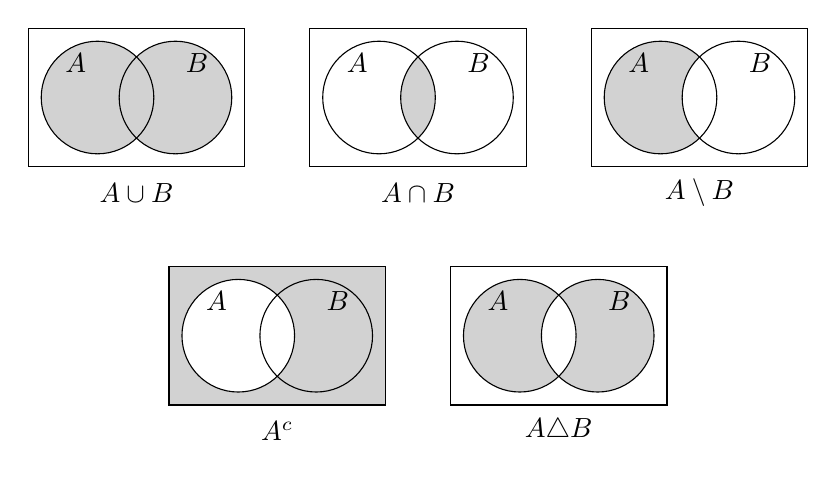
\begin{tikzpicture}[scale=.55]
\begin{scope}[shift={(0,0)}]
\fill[gray!35] (0,0) circle(1.3);\fill[gray!35] (1.8,0) circle(1.3);
\draw (-1.6,-1.6) rectangle(3.4,1.6);\draw (0,0) circle(1.3);\draw(1.8,0) circle(1.3);
\node at(-.5,.8){$A$};\node at(2.3,.8){$B$};\node at(.9,-2.2){$A\cup B$};
\end{scope}
\begin{scope}[shift={(6.5,0)}]
\begin{scope}\clip (0,0) circle(1.3);\fill[gray!35] (1.8,0) circle(1.3);\end{scope}
\draw (-1.6,-1.6) rectangle(3.4,1.6);\draw (0,0) circle(1.3);\draw(1.8,0) circle(1.3);
\node at(-.5,.8){$A$};\node at(2.3,.8){$B$};\node at(.9,-2.2){$A\cap B$};
\end{scope}
\begin{scope}[shift={(13,0)}]
\fill[gray!35] (0,0) circle(1.3);\fill[white] (1.8,0) circle(1.3);
\draw (-1.6,-1.6) rectangle(3.4,1.6);\draw (0,0) circle(1.3);\draw(1.8,0) circle(1.3);
\node at(-.5,.8){$A$};\node at(2.3,.8){$B$};\node at(.9,-2.2){$A\setminus B$};
\end{scope}
\begin{scope}[shift={(3.25,-5.5)}]
\fill[gray!35] (-1.6,-1.6) rectangle(3.4,1.6);\fill[white] (0,0) circle(1.3);
\draw (-1.6,-1.6) rectangle(3.4,1.6);\draw (0,0) circle(1.3);\draw(1.8,0) circle(1.3);
\node at(-.5,.8){$A$};\node at(2.3,.8){$B$};\node at(.9,-2.2){$A^c$};
\end{scope}
\begin{scope}[shift={(9.75,-5.5)}]
\fill[gray!35] (0,0) circle(1.3);\fill[gray!35] (1.8,0) circle(1.3);
\begin{scope}\clip (0,0) circle(1.3);\fill[white] (1.8,0) circle(1.3);\end{scope}
\draw (-1.6,-1.6) rectangle(3.4,1.6);\draw (0,0) circle(1.3);\draw(1.8,0) circle(1.3);
\node at(-.5,.8){$A$};\node at(2.3,.8){$B$};\node at(.9,-2.2){$A\triangle B$};
\end{scope}
\end{tikzpicture}
\end{center}
图中矩形表示全集 $U$，阴影表示相应运算的结果。集合补与命题否定一样依赖指定背景。

\subsection{集合语言的符号化}
集合包含对应全称条件，交集为空对应不存在共同对象。设 $F,S$ 为一、二年级学生集，$R,M$ 为计算机系、数学系学生集，$T,L,P$ 为选修离散数学、爱好文学、爱好体育的学生集：
\begin{align*}
\text{计算机系二年级学生都选修离散数学：}&\quad R\cap S\subseteq T,\\
\text{数学系一年级学生都不选修离散数学：}&\quad M\cap F\cap T=\varnothing,\\
\text{数学系学生都爱好文学或体育：}&\quad M\subseteq L\cup P,\\
\text{只有一、二年级学生才爱好体育：}&\quad P\subseteq F\cup S.
\end{align*}
“选修离散数学的只有数学系或计算机系二年级学生”若意为这两个系的二年级学生，写为 $T\subseteq(M\cup R)\cap S$；若意为数学系全部学生或计算机系二年级学生，写为 $T\subseteq M\cup(R\cap S)$。自然语言范围存在歧义时应先澄清结构再列式。

\subsection{广义并、广义交与运算层次}
对以集合为元素的非空集合族 $\mathcal A$，定义
\begin{align*}
\bigcup\mathcal A&=\{x\mid\exists Z(Z\in\mathcal A\land x\in Z)\},\\
\bigcap\mathcal A&=\{x\mid\forall Z(Z\in\mathcal A\to x\in Z)\}.
\end{align*}
有限集合族满足 $\bigcup\{A_1,\ldots,A_n\}=A_1\cup\cdots\cup A_n$，广义交同理。索引族可写为 $\bigcup_{i\in I}A_i$ 和 $\bigcap_{i\in I}A_i$；属于广义并意味着至少属于一项，属于广义交意味着属于每一项。
\example{减少一层集合括号}
\[
\bigcup\{\{1\},\{1,2\},\{1,2,3\}\}=\{1,2,3\},\qquad
\bigcap\{\{1\},\{1,2\},\{1,2,3\}\}=\{1\}.
\]
若 $A$ 是集合，$\bigcup\{A\}=\bigcap\{A\}=A$。单个原子对象一般不能直接参与广义并交；“去掉括号一层”只是便于记忆，严格含义取决于元素也是集合。

$\bigcup\varnothing=\varnothing$。课件在未固定全集的集合论语境下不定义 $\bigcap\varnothing$；若预先固定 $U$ 并将交限制为 $U$ 中满足条件的元素，则可约定空族交为 $U$。两种约定的背景不同，不应混用。

课件将广义并交、幂集和补列为优先的运算，嵌套时由内到外（书写上从右向左）计算；普通 $\cup,\cap,\setminus,\triangle$ 的混合次序用括号确定。
\example{多层运算}
设 $\mathcal A=\{\{a\},\{a,b\}\}$，其中 $a,b$ 本身为集合，则
\begin{align*}
\bigcap(\bigcup\mathcal A)
\cup\bigl(\bigcup(\bigcup\mathcal A)\setminus\bigcup(\bigcap\mathcal A)\bigr)
&=(a\cap b)\cup((a\cup b)\setminus a)\\
&=(a\cap b)\cup(b\setminus a)=b.
\end{align*}
若 $a,b$ 不是集合，上述广义运算未必有意义。

广义德摩根律在固定 $U$ 中为
\[
\left(\bigcup_{i\in I}A_i\right)^c=\bigcap_{i\in I}A_i^c,\qquad
\left(\bigcap_{i\in I}A_i\right)^c=\bigcup_{i\in I}A_i^c.
\]

\subsection{集合运算的算律}
\begin{longtable}{p{0.18\linewidth}p{0.75\linewidth}}
\toprule 名称 & 恒等式\\\midrule\endhead
交换律 & $A\cup B=B\cup A$；$A\cap B=B\cap A$\\
结合律 & $(A\cup B)\cup C=A\cup(B\cup C)$；\newline $(A\cap B)\cap C=A\cap(B\cap C)$\\
幂等律 & $A\cup A=A$；$A\cap A=A$\\
分配律 & $A\cup(B\cap C)=(A\cup B)\cap(A\cup C)$；\newline $A\cap(B\cup C)=(A\cap B)\cup(A\cap C)$\\
吸收律 & $A\cup(A\cap B)=A$；$A\cap(A\cup B)=A$\\
补元律 & $A\cup A^c=U$；$A\cap A^c=\varnothing$\\
双重补 & $(A^c)^c=A$\\
德摩根律 & $(A\cup B)^c=A^c\cap B^c$；$(A\cap B)^c=A^c\cup B^c$\\
差的德摩根式 & $A\setminus(B\cup C)=(A\setminus B)\cap(A\setminus C)$；\newline $A\setminus(B\cap C)=(A\setminus B)\cup(A\setminus C)$\\
零律 & $A\cup U=U$；$A\cap\varnothing=\varnothing$\\
同一律 & $A\cup\varnothing=A$；$A\cap U=A$\\
补的特例 & $\varnothing^c=U$；$U^c=\varnothing$\\\bottomrule
\end{longtable}
对称差还满足
\begin{align*}
A\triangle B&=B\triangle A,\\
(A\triangle B)\triangle C&=A\triangle(B\triangle C),\\
A\triangle A&=\varnothing,\qquad A\triangle\varnothing=A,\\
(A\triangle B)\triangle B&=A,\\
A\cap(B\triangle C)&=(A\cap B)\triangle(A\cap C).
\end{align*}
对称差符合“奇数次出现保留、偶数次出现消去”的规律。差一般不交换、不结合；并不能任意替代交来对对称差分配。
\example{差不满足结合律}
取 $A=B=C=\{1\}$，则 $(A\setminus B)\setminus C=\varnothing$，而 $A\setminus(B\setminus C)=\{1\}$。因此集合差的括号不能随意省略。

\subsection{包含的等价条件与单调性}
\[
A\subseteq B\Longleftrightarrow A\cup B=B
\Longleftrightarrow A\cap B=A
\Longleftrightarrow A\setminus B=\varnothing.
\]
还常用
\[
A\cap B=\varnothing\Longleftrightarrow A\setminus B=A,\qquad
A=B\Longleftrightarrow A\triangle B=\varnothing.
\]
若 $A\subseteq B$，则 $A\cup C\subseteq B\cup C$、$A\cap C\subseteq B\cap C$、$A\setminus C\subseteq B\setminus C$，并有 $B^c\subseteq A^c$。差对第二个变量方向相反：$C\setminus B\subseteq C\setminus A$。

\example{完整证明包含的等价条件}
若 $A\subseteq B$，则 $A\cup B=B$。由 $A\cup B=B$ 与吸收律得 $A=A\cap(A\cup B)=A\cap B$。若 $A\cap B=A$，则任何 $A$ 的元素都在 $B$，故 $A\setminus B=\varnothing$。若 $A\setminus B=\varnothing$，就不存在属于 $A$ 而不属于 $B$ 的元素，即 $A\subseteq B$。首尾连成闭环，四个条件等价。

\subsection{集合包含与恒等式的证明方法}
\term{元素法（命题演算法）：}证明 $X\subseteq Y$ 时，任取 $x\in X$，根据定义推出 $x\in Y$；证明 $X=Y$ 时，可以双向包含，也可写出 $x\in X\Longleftrightarrow\cdots\Longleftrightarrow x\in Y$。

\term{包含传递法：}寻找中间集合 $T$，由 $X\subseteq T\subseteq Y$ 得 $X\subseteq Y$。例如 $A\setminus B\subseteq A\subseteq A\cup B$。

\term{等价条件法：}把包含转换为并、交、差等式再证明。\term{算律演算法（等式替换法）：}逐步使用已知集合算律，将一侧变为另一侧。\term{运算法：}对已知包含或等式同时取并、交、差、补等合法运算，得到新关系；取补时要注意包含方向反转。

\term{反证法：}否定 $X\subseteq Y$，即假设存在 $x\in X\setminus Y$，导出矛盾。否定 $X=Y$ 时，存在 $x$ 恰好属于二者之一，需覆盖两种方向。
\example{幂集与包含}
证明 $A\subseteq B\Longleftrightarrow\mathcal P(A)\subseteq\mathcal P(B)$。
正向：任取 $X\in\mathcal P(A)$，则 $X\subseteq A\subseteq B$，故 $X\in\mathcal P(B)$。
逆向：任取 $x\in A$，则 $\{x\}\in\mathcal P(A)\subseteq\mathcal P(B)$，故 $\{x\}\subseteq B$，即 $x\in B$。

\example{由分块包含恢复整体包含}
若 $A\cap C\subseteq B\cap C$ 且 $A\setminus C\subseteq B\setminus C$，则对两式取并：
\[
(A\cap C)\cup(A\setminus C)\subseteq
(B\cap C)\cup(B\setminus C).
\]
因为每个集合都分成位于 $C$ 内外的两块，两侧分别等于 $A,B$，故 $A\subseteq B$。

\example{由并、交等式恢复原集合}
若 $A\cup B=A\cup C$ 且 $A\cap B=A\cap C$，证明 $B=C$。
用算律有
\begin{align*}
B&=B\cap(A\cup B)=B\cap(A\cup C)\\
&=(B\cap A)\cup(B\cap C)\\
&=(A\cap C)\cup(B\cap C)=(A\cup B)\cap C\\
&=(A\cup C)\cap C=C.
\end{align*}
也可将两条已知式相减，得到 $A\triangle B=A\triangle C$，再对两边与 $A$ 取对称差，利用消去律得到 $B=C$。

\example{恒等式的元素证明}
\begin{align*}
x\in A\setminus(B\cup C)
&\Longleftrightarrow x\in A\land\neg(x\in B\lor x\in C)\\
&\Longleftrightarrow(x\in A\land x\notin B)\land(x\in A\land x\notin C)\\
&\Longleftrightarrow x\in(A\setminus B)\cap(A\setminus C).
\end{align*}
由于 $x$ 任意，得到 $A\setminus(B\cup C)=(A\setminus B)\cap(A\setminus C)$。证明集合恒等式的核心是利用逻辑等值，而非仅观察特定图形。

\subsection{集合等式的充分必要条件}
求等式成立的条件时，先推导必要条件，再验证它确实充分。
\begin{center}
\begin{tabularx}{\linewidth}{Y Y}
\toprule 等式 & 充分必要条件\\\midrule
$A\setminus B=B$ & $A=B=\varnothing$\\
$A\setminus B=B\setminus A$ & $A=B$\\
$A\cap B=A\cup B$ & $A=B$\\
$A\triangle B=A$ & $B=\varnothing$\\
$A\setminus B=A$ & $A\cap B=\varnothing$\\
$A\cap B=B$ & $B\subseteq A$\\\bottomrule
\end{tabularx}
\end{center}
\example{课件习题的四个条件推导}
若 $A\setminus B=B$，左侧与 $B$ 不相交，故 $B=\varnothing$，代回得 $A=\varnothing$。若 $A\setminus B=B\setminus A$，两侧相互不交又相等，因此都为空，得到相互包含，故 $A=B$。若 $A\cap B=A\cup B$，则 $A\subseteq A\cup B=A\cap B\subseteq B$，交换角色得 $B\subseteq A$，故 $A=B$。若 $A\triangle B=A$，两侧与 $A$ 取对称差，得 $B=\varnothing$。各条件代回原式均成立，因而也是充分条件。

\subsection{有限集合的计数与容斥原理}
对有限集合，$|A\setminus B|=|A|-|A\cap B|$，$|A^c|=|U|-|A|$。
\term{两集合容斥公式}为
\[
|A\cup B|=|A|+|B|-|A\cap B|.
\]
\term{三集合容斥公式}为
\begin{align*}
|A\cup B\cup C|
={}&|A|+|B|+|C|\\
&-|A\cap B|-|A\cap C|-|B\cap C|+|A\cap B\cap C|.
\end{align*}
\term{一般容斥公式}为
\[
\left|\bigcup_{i=1}^{m}A_i\right|
=\sum_{\varnothing\ne J\subseteq\{1,\ldots,m\}}
(-1)^{|J|+1}\left|\bigcap_{j\in J}A_j\right|.
\]
若求 $U$ 中不属于任何 $A_i$ 的人数，用 $|U|$ 减去并集基数。

证明思路：某个属于恰好 $r\ge1$ 个集合的元素，在右侧贡献
\[
\binom r1-\binom r2+\cdots+(-1)^{r+1}\binom rr=1,
\]
这是 $(1-1)^r=0$ 的结果。因此每个并集元素恰好计一次，不在并集中的元素贡献为 $0$。

对三个集合令 $S_1=|A|+|B|+|C|$，$S_2=|A\cap B|+|A\cap C|+|B\cap C|$，$S_3=|A\cap B\cap C|$，则恰好属于三个、两个、一个集合的元素数分别为
\[
N_3=S_3,\quad N_2=S_2-3S_3,\quad N_1=S_1-2S_2+3S_3.
\]
“既属于 $A$ 又属于 $B$”的计数通常包括同时属于 $C$ 的对象，不能直接理解为“恰好属于两类”。

\example{两类兴趣人数}
$20$ 名学生中 $10$ 人爱好音乐、$8$ 人爱好美术、$6$ 人两者都爱好。至少爱好一类者有 $10+8-6=12$ 人；两类都不爱好者有 $20-12=8$ 人。只爱好音乐者 $4$ 人，只爱好美术者 $2$ 人，恰好爱好一类者 $6$ 人。

\example{整数的整除筛选}
求 $1$ 至 $1000$ 中，均不能被 $5,6,8$ 中任一个整除的整数数目。令 $A,B,C$ 为分别被 $5,6,8$ 整除的集合。被若干数同时整除，等价于被它们的最小公倍数整除：
\begin{align*}
|A|&=\lfloor1000/5\rfloor=200,\quad
|B|=\lfloor1000/6\rfloor=166,\quad |C|=125,\\
|A\cap B|&=\lfloor1000/30\rfloor=33,\quad
|A\cap C|=25,\quad |B\cap C|=41,\\
|A\cap B\cap C|&=\lfloor1000/120\rfloor=8.
\end{align*}
故所求为 $1000-(200+166+125)+(33+25+41)-8=600$。交集的分母应取最小公倍数，不能总是把除数直接相乘。

\example{四种语言及“只会一种”的计数}
$24$ 人每人至少会一种外语。英语 $13$ 人、日语 $5$ 人、德语 $10$ 人、法语 $9$ 人；英语与日语交集 $2$ 人，英语与德语、英语与法语、德语与法语交集均为 $4$ 人；会日语者不会德语、法语。

设同时会英、德、法者为 $t$。其他三重及四重交集均为空，由容斥有
\[
24=13+5+10+9-(2+4+4+4)+t,
\]
得 $t=1$。只会英语、日语、德语、法语的人数分别为
\[
13-2-4-4+1=4,\quad5-2=3,\quad10-4-4+1=3,\quad9-4-4+1=2.
\]
因此只会一种语言者 $12$ 人，恰好会两种者 $2+3(4-1)=11$ 人，恰好会三种者 $1$ 人，合计 $24$ 人。

\subsection{计数对象与等同规则}
\example{三个硬币的结果集合}
若三个硬币有编号或按抛掷次序区分，结果集合为
\[
\{HHH,HHT,HTH,HTT,THH,THT,TTH,TTT\},
\]
共 $8$ 个元素。若只关心正面个数、忽略硬币身份，则归并为 $0,1,2,3$ 个正面四类。集合的无序性不意味着字符串内部的顺序也无意义；是否归并由题目的结果定义决定。

\example{三个区域的旋转着色}
将正三角形的三个可循环轮换的区域用黑、白两色着色，位置固定时有 $2^3=8$ 种。若旋转重合视为相同，则按黑色区域个数分为 $0,1,2,3$ 四类。在此三区域模型中同黑色个数的方案可互相旋转重合，因此有 $4$ 类；对更多区域不能仅按黑色个数自动归并。

\exercise
\begin{enumerate}
\begin{samepage}
\item 判断 $\varnothing\subseteq\varnothing$、$\varnothing\in\varnothing$、$\varnothing\subseteq\{\varnothing\}$、$\varnothing\in\{\varnothing\}$。\\
\term{解：}依次为真、假、真、真。若 $A=\{a,b,c,\{a,b\}\}$，则 $\{a,b\}\subseteq A$ 与 $\{a,b\}\in A$ 同时成立。
\end{samepage}
\begin{samepage}
\item 设 $S_1=\{1,\ldots,9\},S_2=\{2,4,6,8\},S_3=\{1,3,5,7,9\},S_4=\{3,4,5\},S_5=\{3,5\}$。限定 $X$ 是这五个候选集合之一，分别求：$X\cap S_5=\varnothing$；$X\subseteq S_4$ 且 $X\cap S_2=\varnothing$；$X\subseteq S_1$ 且 $X\nsubseteq S_3$；$X\setminus S_3=\varnothing$；$X\subseteq S_3$ 且 $X\nsubseteq S_1$。\\
\term{解：}依次为 $S_2$；$S_5$；$S_1,S_2,S_4$；$S_3,S_5$；无候选。若不限制为候选，前四题通常有更多解，不能据上述条件断言唯一集合。
\end{samepage}
\begin{samepage}
\item 判断“$A\setminus B=A$ 当且仅当 $B=\varnothing$”。\\
\term{解：}错误，必要条件应为 $A\cap B=\varnothing$。反例 $A=\{1\},B=\{2\}$。
\end{samepage}
\begin{samepage}
\item 判断“$A\triangle A=A$”和“$A\cap B=B$ 则 $A=U$”。\\
\term{解：}均错误。前者通常为 $\varnothing$，取 $A=\{1\}$ 可反驳；后者只要求 $B\subseteq A$，取 $U=\{1,2\},A=B=\{1\}$ 可反驳。
\end{samepage}
\begin{samepage}
\item 若 $x$ 是集合且 $A=\{x\}\cup x$，证明 $x\in A$ 且 $x\subseteq A$。\\
\term{解：}$x\in\{x\}\subseteq A$，故属于关系成立；$x\subseteq\{x\}\cup x=A$，故包含关系也成立。
\end{samepage}
\begin{samepage}
\item 证明 $\mathcal P(A\cap B)=\mathcal P(A)\cap\mathcal P(B)$，并判断幂集是否同样对并分配。\\
\term{解：}$X\subseteq A\cap B$ 当且仅当 $X\subseteq A$ 且 $X\subseteq B$。对并一般只有 $\mathcal P(A)\cup\mathcal P(B)\subseteq\mathcal P(A\cup B)$；取 $A=\{1\},B=\{2\}$，子集 $\{1,2\}$ 仅属于右侧。
\end{samepage}
\begin{samepage}
\item $50$ 人中参加三项活动的人数分别为 $25,20,18$，两两交集人数分别为 $10,8,6$，三重交集为 $3$。求未参加者、恰好参加两项者和恰好参加一项者。\\
\term{解：}并集人数为 $25+20+18-10-8-6+3=42$，未参加者 $8$；恰好两项者 $24-9=15$；恰好一项者 $63-48+9=24$。再加三项者 $3$，总数为 $42$。
\end{samepage}
\end{enumerate}
\note{集合的括号层次决定元素身份；幂集元素是子集；广义运算的输入是集合族；容斥中的交集默认包含更高重交集，计数前须明确全集与等同规则。}
\chapterpage{二元关系}
二元关系用有序对描述对象之间的联系。等价关系将对象分类，偏序关系描述对象之间的次序。本章依据第七章 7.6--7.7 节及其习题课整理；为使本章可独立阅读，先补充关系表示、运算、性质和闭包的必要定义。

\subsection{有序对、笛卡尔积与二元关系}
\term{有序对} $\langle a,b\rangle$ 的两个分量有先后之分，且
\[
\langle a,b\rangle=\langle c,d\rangle\quad\Longleftrightarrow\quad a=c\land b=d.
\]
集合 $A,B$ 的\term{笛卡尔积}为 $A\times B=\{\langle a,b\rangle\mid a\in A,b\in B\}$。从 $A$ 到 $B$ 的二元关系是 $A\times B$ 的任一子集；$A$ 上的二元关系是 $A\times A$ 的子集。$\langle x,y\rangle\in R$ 简记为 $xRy$。

设 $|A|=m,|B|=n$，则 $|A\times B|=mn$，从 $A$ 到 $B$ 的关系共有 $2^{mn}$ 个。恒等关系 $I_A=\{\langle a,a\rangle\mid a\in A\}$，全域关系 $E_A=A\times A$。空关系 $\varnothing$ 与承载关系的集合 $A$ 应分开说明。

\subsection{关系的三种表示与定义域、值域}
关系可用集合表达式、关系矩阵和关系图表示。固定有限集合 $A=\{a_1,\ldots,a_n\}$ 的顺序后，关系矩阵 $M_R=(r_{ij})$ 定义为
\[
r_{ij}=1\Longleftrightarrow a_iRa_j,\qquad r_{ij}=0\Longleftrightarrow\neg(a_iRa_j).
\]
行是起点、列是终点。关系图在每个元素处画一个顶点，$a_iRa_j$ 时画有向边 $a_i\to a_j$；$a_iRa_i$ 对应自环。
\begin{align*}
\operatorname{dom}R&=\{x\mid\exists y\,(xRy)\},\\
\operatorname{ran}R&=\{y\mid\exists x\,(xRy)\},\\
\operatorname{fld}R&=\operatorname{dom}R\cup\operatorname{ran}R.
\end{align*}
定义域不一定是题目指定的整个 $A$，值域也不一定是整个 $B$。

\subsection{逆、合成、幂、限制与像}
\term{逆关系} $R^{-1}=\{\langle y,x\rangle\mid xRy\}$，其矩阵为 $M_R$ 的转置。
本章沿用课件的合成顺序：$R\circ S$ 表示\term{先沿 $R$，再沿 $S$}，即
\[
x(R\circ S)z\quad\Longleftrightarrow\quad\exists y\,(xRy\land ySz).
\]
不同教材可能采用相反的书写约定，运算时必须先核对定义。课件习题给出的 $R\circ S$ 结果与上述顺序一致。

在本约定下，$R^0=I_A$，$R^{n+1}=R^n\circ R$；$xR^ny$ 表示存在长度为 $n$ 的有向行走，从 $x$ 到 $y$。合成满足结合律，一般不满足交换律，且
\[
(R\circ S)^{-1}=S^{-1}\circ R^{-1}.
\]
关系矩阵的合成使用布尔乘法：$c_{ij}=\bigvee_k(r_{ik}\land s_{kj})$，不能把普通矩阵乘法中的正整数结果直接作为关系矩阵元素。

若 $C\subseteq A$，则
\begin{align*}
R\mathbin{\upharpoonright}C&=\{\langle x,y\rangle\in R\mid x\in C\},\\
R[C]&=\{y\mid\exists x\in C\,(xRy)\}.
\end{align*}
前者是按第一分量限制关系，后者是 $C$ 在 $R$ 下的像；若要得到 $C$ 上的诱导关系，则应取 $R\cap(C\times C)$。

\subsection{关系的基本性质与闭包}
对 $R\subseteq A\times A$，各性质的量词范围均为 $A$。
\begin{longtable}{p{0.16\linewidth}p{0.77\linewidth}}
\toprule 性质 & 定义\\\midrule\endhead
自反 & $\forall x\;(xRx)$\\
反自反 & $\forall x\;\neg(xRx)$\\
对称 & $\forall x\forall y\;(xRy\to yRx)$\\
反对称 & $\forall x\forall y\;((xRy\land yRx)\to x=y)$\\
传递 & $\forall x\forall y\forall z\;((xRy\land yRz)\to xRz)$\\\bottomrule
\end{longtable}
反对称并非“不对称”：恒等关系既对称又反对称。传递性要求每条两步路径都有对应的直达关系，不能仅检查某一组三个元素。证明性质时任取相关元素，展开定义；否定性质时给出违反量词条件的具体反例。

\term{闭包}是在包含原关系的前提下，满足指定性质的最小关系。自反、对称、传递闭包分别为
\[
r(R)=R\cup I_A,\qquad s(R)=R\cup R^{-1},\qquad
t(R)=\bigcup_{n\ge1}R^n.
\]
传递闭包包含正长度路径的全部可达关系；只有存在正长度回路时，才会因此加入相应自环。它与自反传递闭包 $I_A\cup t(R)$ 不同。若 $|A|=n\ge1$，则 $t(R)=R\cup\cdots\cup R^n$。

\example{关系运算与三类闭包（习题课第 1 题）}
设 $A=\{1,2,3\}$，$R=\{\langle x,y\rangle\in A^2\mid x+2y\le6\}$，$S=\{\langle1,2\rangle,\langle1,3\rangle,\langle2,2\rangle\}$。逐项枚举得
\begin{align*}
R&=\{(1,1),(1,2),(2,1),(2,2),(3,1)\},\\
R^{-1}&=\{(1,1),(1,2),(1,3),(2,1),(2,2)\},\\
\operatorname{dom}R&=\{1,2,3\},\quad\operatorname{ran}R=\{1,2\},\quad\operatorname{fld}R=A,\\
R\circ S&=\{(1,2),(1,3),(2,2),(2,3),(3,2),(3,3)\}.
\end{align*}
例如 $3R1$ 且 $1S3$，故 $(3,3)\in R\circ S$。为节省篇幅，这里用 $(x,y)$ 表示有序对。由 $3\to1\to2$，$R^2$ 比 $R$ 仅多 $(3,2)$，以后不再增加，故
\begin{align*}
R^3=t(R)&=R\cup\{(3,2)\},\\
r(R)&=R\cup\{(3,3)\},\\
s(R)&=R\cup\{(1,3)\}.
\end{align*}
特别地，$t(R)$ 不含 $(3,3)$，因为没有从 $3$ 回到 $3$ 的正长度路径。

\subsection{等价关系及其判定}
$A$ 上自反、对称且传递的关系称为\term{等价关系}，常记作 $\sim$。它表达对象在某一分类标准下的相同，而不要求对象本身相等。

固定标准下的同龄、同寝室关系，三角形的相似、全等关系，以及命题公式的逻辑等值关系，均为典型例子。$I_A$ 与 $E_A$ 也是等价关系；“年龄差不超过一岁”则不一定传递，不能作为等价关系。

\example{模 $m$ 同余是等价关系}
固定正整数 $m$，在 $\mathbb Z$ 上定义 $x\sim y\Longleftrightarrow m\mid(x-y)$。
由 $x-x=0$ 得自反性。若 $x-y=km$，则 $y-x=(-k)m$，得对称性。若 $x-y=km$、$y-z=\ell m$，则 $x-z=(k+\ell)m$，得传递性。因此模 $m$ 同余是等价关系。

这里 $m$ 必须预先固定，不能对每一对整数任意换用不同的模数。$m=1$ 时所有整数同属一类；$m>1$ 时有 $m$ 个不同余数类。

\subsection{等价类、代表元与商集}
若 $R$ 是 $A$ 上的等价关系，$a\in A$，则
\[
[a]_R=\{x\in A\mid aRx\}
\]
称为 $a$ 的\term{等价类}，$a$ 称为该类的一个代表元。由对称性，定义也可写成 $\{x\in A\mid xRa\}$。有
\begin{enumerate}
\item $a\in[a]_R$，故每个等价类非空。
\item $aRb\Longleftrightarrow[a]_R=[b]_R$。
\item 两个等价类要么相等，要么不相交。
\item 所有等价类的并为 $A$。
\end{enumerate}
\term{证明：}若 $aRb$，任取 $x\in[a]_R$，由 $bRa$、$aRx$ 得 $bRx$，故 $[a]_R\subseteq[b]_R$，反向同理。若两类有公共元素 $c$，则由 $aRc$ 和 $cRb$ 得 $aRb$，于是两类相等。最后，每个 $a$ 属于自己的类，且每个类包含于 $A$，所以并集恰为 $A$。

以所有不同等价类为元素的集合称为\term{商集}：
\[
A/R=\{[a]_R\mid a\in A\}.
\]
商集的元素是集合，不能把代表元集合与商集混同。对于非空 $A$，$A/I_A=\{\{a\}\mid a\in A\}$，$A/E_A=\{A\}$。

\example{同余类与有限集合上的模 $3$ 分类}
在 $A=\{1,\ldots,8\}$ 上按模 $3$ 同余分类，得
\[
A/R=\bigl\{\{1,4,7\},\{2,5,8\},\{3,6\}\bigr\}.
\]
代表元可以选 $1,2,3$，也可以选 $4,5,6$，但商集仍是上述三个集合组成的集合。在 $\mathbb Z$ 上按模 $m$ 同余分类，则
\[
[r]=r+m\mathbb Z=\{r+km\mid k\in\mathbb Z\},\quad
\mathbb Z/R=\{[0],[1],\ldots,[m-1]\}.
\]
模 $4$ 时为 $4\mathbb Z,1+4\mathbb Z,2+4\mathbb Z,3+4\mathbb Z$；模 $2$ 时为偶整数类和奇整数类。

\example{等价关系的集合、矩阵与关系图}
设 $X=\{0,1,2,3,4\}$，$xRy\Longleftrightarrow2\mid(x-y)$。按 $0,1,2,3,4$ 排列，
\[
M_R=\begin{pmatrix}
1&0&1&0&1\\0&1&0&1&0\\1&0&1&0&1\\0&1&0&1&0\\1&0&1&0&1
\end{pmatrix},\qquad
X/R=\bigl\{\{0,2,4\},\{1,3\}\bigr\}.
\]
关系集合为 $R=\{0,2,4\}^2\cup\{1,3\}^2$。关系图中每点都有自环，同类的任意两不同点间均有双向边，不同类之间无边。
\begin{center}
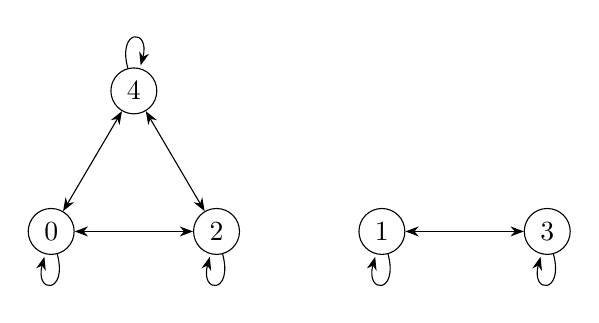
\begin{tikzpicture}[>=Stealth,every node/.style={circle,draw,inner sep=3pt},scale=1.05]
\node (z) at (0,0) {$0$};\node (t) at (2,0) {$2$};\node (f) at (1,1.7) {$4$};
\node (o) at (4,0) {$1$};\node (h) at (6,0) {$3$};
\foreach \u/\v in {z/t,t/f,f/z,o/h}\draw[<->] (\u)--(\v);
\foreach \u in {z,t,o,h}\path[->] (\u) edge[loop below] (\u);
\path[->] (f) edge[loop above] (f);
\end{tikzpicture}
\end{center}
若把同类元素相邻排列，矩阵呈对角全 $1$ 方块，不同方块之间全 $0$。这给出有限等价关系的另一种检查方式。

\subsection{划分与等价关系的一一对应}
集合 $A$ 的一个\term{划分}是集合族 $\pi\subseteq\mathcal P(A)$，满足
\[
\varnothing\notin\pi,\quad
B,C\in\pi,\ B\ne C\Rightarrow B\cap C=\varnothing,\quad
\bigcup\pi=A.
\]
$\pi$ 的元素称为划分块。三个条件分别要求块非空、不同块互斥、覆盖全体元素。对于空集，唯一划分是空族 $\varnothing$，不是 $\{\varnothing\}$。

\example{判断一个集合族是否构成划分}
对 $A=\{a,b,c,d\}$，$\{\{a,b\},\{c\},\{d\}\}$ 是划分。
$\{\{a\},\{a,b,c,d\}\}$ 中两块相交，故不是划分。
$\{\{a,b\},\{c\}\}$ 漏掉 $d$，含 $\varnothing$ 的集合族也不符合要求。元素集合、块和由块构成的划分共有三个层次，不能省略括号。

\term{对应定理：}等价关系 $R$ 确定划分 $\pi_R=A/R$；反之，划分 $\pi$ 确定等价关系
\[
R_\pi=\bigcup_{B\in\pi}(B\times B),\qquad
xR_\pi y\Longleftrightarrow\exists B\in\pi\;(x,y\in B).
\]
\term{证明：}由等价类的性质，$\pi_R$ 满足划分的三个条件。对 $R_\pi$，每个元素在某一块中，故自反；同块关系对称；若 $x,y$ 同块、$y,z$ 同块，这两块有公共元素 $y$，必为同一块，故 $x,z$ 同块，得到传递性。

从 $R$ 出发再构造 $R_{\pi_R}$，有 $xR_{\pi_R}y\Longleftrightarrow[x]_R=[y]_R\Longleftrightarrow xRy$，因此回到 $R$。从 $\pi$ 出发，$[x]_{R_\pi}$ 恰为包含 $x$ 的唯一划分块，因此也回到原划分。两个构造互为逆过程。

\example{由等价关系求商集的步骤}
令 $A=\{1,2,3,4\}$，$R=\{1,2\}^2\cup\{3,4\}^2$。先取 $1$，得到 $[1]=\{1,2\}$；再从尚未归类的 $A\setminus[1]=\{3,4\}$ 中取 $3$，得到 $[3]=\{3,4\}$。两类之并为 $A$，故
\[
A/R=\bigl\{\{1,2\},\{3,4\}\bigr\}.
\]
一般步骤是：选择尚未归类的元素，求其等价类，加入结果并标记其中所有元素，直到没有剩余元素。课件第 28 页第二步应在已求类的\term{外部}选择新代表元。

若有限划分的块大小为 $n_1,\ldots,n_k$，则
\[
|A/R|=k,\qquad |A|=\sum_{i=1}^kn_i,\qquad |R|=\sum_{i=1}^kn_i^2.
\]
最后一式计算的是有序对数，而不是等价类数。

\subsection{等价关系计数与划分细分}
$n$ 元集合上等价关系的个数等于其划分个数。对 $|A|=4$，按块大小分类：
\begin{center}
\begin{tabular}{c c l}
\toprule 块大小 & 个数 & 计算依据\\\midrule
$1+1+1+1$ & $1$ & 全为单点块\\
$2+1+1$ & $6$ & 选择二元素块：$\binom42$\\
$2+2$ & $3$ & $\binom42/2$，两块不编号\\
$3+1$ & $4$ & 选择单点块：$\binom41$\\
$4$ & $1$ & 仅一个块\\\bottomrule
\end{tabular}
\end{center}
总数为 $1+6+3+4+1=15$。三元素集相应为 $1+3+1=5$。

对于 $A$ 的两个划分，若 $\pi_1$ 的每一块都包含于 $\pi_2$ 的某一块，称 $\pi_1$\term{细分} $\pi_2$，记 $\pi_1\le\pi_2$。若还不相等，称真细分。例如
\[
\{\{a\},\{b\},\{c\},\{d\}\}
\le\{\{a,b\},\{c\},\{d\}\}
\le\{\{a,b,c\},\{d\}\}.
\]
细分关系不是集合族的普通包含关系。与对应等价关系的联系是
\[
R_1\subseteq R_2\quad\Longleftrightarrow\quad\pi_{R_1}\le\pi_{R_2}.
\]
\term{证明：}若 $R_1\subseteq R_2$，则每个 $[a]_{R_1}\subseteq[a]_{R_2}$。反之，若划分细分，$xR_1y$ 意味着二者所在的 $R_1$ 类包含在同一 $R_2$ 类中，故 $xR_2y$。因此关系中的有序对越少，分类越细。$I_A$ 对应最细划分，非空 $A$ 上的 $E_A$ 对应最粗划分。

\subsection{偏序、可比、全序与严格偏序}
集合 $A$ 上自反、反对称且传递的关系称为\term{偏序关系}，记为 $\preceq$；$\langle A,\preceq\rangle$ 称为\term{偏序集}。符号 $x\preceq y$ 表示在指定次序下 $x$ 先于或等于 $y$，未必表示数值大小。

实数上的 $\le$ 与 $\ge$、正整数上的整除 $\mid$、幂集上的包含 $\subseteq$，均为偏序。整除关系在\term{正整数}上反对称；若在全部整数上直接使用，则 $1\mid-1$、$-1\mid1$ 而 $1\ne-1$，反对称性不成立。

若 $x\preceq y$ 或 $y\preceq x$，称两者\term{可比}；否则不可比。任意两元素均可比的偏序称为\term{全序}（线序）。例如数值 $\le$ 是全序，而 $2,3$ 在整除次序下不可比，所以正整数整除不是全序。

定义 $x\prec y\Longleftrightarrow(x\preceq y\land x\ne y)$，得到相应\term{严格偏序}，其性质是反自反和传递。严格偏序本身不满足自反性，不能直接当作本章定义的非严格偏序。

\subsection{覆盖关系与哈斯图}
若 $x\prec y$，且不存在 $z\in A$ 满足 $x\prec z\prec y$，称\term{$y$ 覆盖 $x$}。记
\[
\operatorname{cov}(A)=\{\langle x,y\rangle\mid y\text{ 覆盖 }x\}.
\]
覆盖取决于承载集合。例如在 $\{1,2,4\}$ 的整除序中 $4$ 不覆盖 $1$，但在 $\{1,4\}$ 中覆盖。

有限偏序的\term{哈斯图}仅画覆盖边：删去自环，删去可由传递性推出的边，把较小元素画在较低处，并省略向上的箭头。两点之间沿边\term{持续向上}可达，才表示前者小于后者；任意方向的折线路径不代表可比，交叉但没有顶点的线也不表示新元素。

从有限哈斯图恢复关系时，加入所有自环及所有向上可达对。哈斯图不要求可比元素有直接边；图上高度相同也不是判定可比性的定义。有限性保证覆盖关系足以恢复原偏序；一般无限偏序未必如此，例如有理数通常次序没有覆盖对。

\example{正因子集合上的整除序}
对 $D_{12}=\{1,2,3,4,6,12\}$，覆盖对为
\[
\{(1,2),(1,3),(2,4),(2,6),(3,6),(4,12),(6,12)\}.
\]
\begin{center}
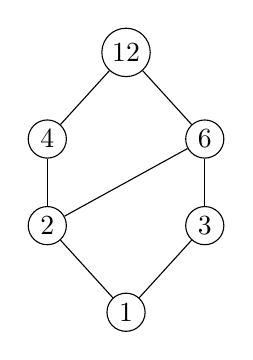
\begin{tikzpicture}[scale=1.0,every node/.style={circle,draw,fill=white,inner sep=2pt}]
\node (a) at (0,0) {$1$};\node (b) at (-1,1.1) {$2$};\node (c) at (1,1.1) {$3$};
\node (d) at (-1,2.2) {$4$};\node (e) at (1,2.2) {$6$};\node (f) at (0,3.3) {$12$};
\foreach \u/\v in {a/b,a/c,b/d,b/e,c/e,d/f,e/f}\draw (\u)--(\v);
\end{tikzpicture}
\end{center}
$1\mid12$，但不画 $1$ 到 $12$ 的直接边，因为这一关系可由路径恢复。$4$ 与 $6$ 虽然数值可比较，但在整除序中不可比。

\example{三种整除序的哈斯图（课件例 7.7.5）}
下图依次表示 $D_8=\{1,2,4,8\}$、$\{2,3,6,12,24,36\}$ 和 $D_{30}$ 上的整除序。
\begin{center}
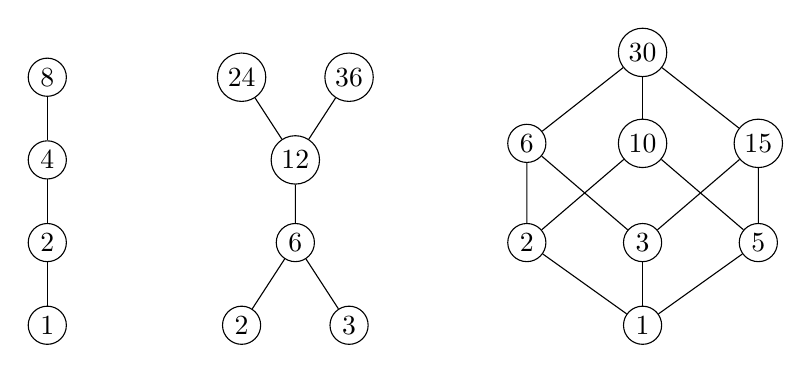
\begin{tikzpicture}[scale=1.05,every node/.style={circle,draw,fill=white,inner sep=2pt}]
\begin{scope}
\node (a) at (0,0) {$1$};\node (b) at (0,1) {$2$};\node (c) at (0,2) {$4$};\node (d) at (0,3) {$8$};
\draw (a)--(b)--(c)--(d);
\end{scope}
\begin{scope}[xshift=3cm]
\node (a) at (-.65,0) {$2$};\node (b) at (.65,0) {$3$};\node (c) at (0,1) {$6$};\node (d) at (0,2) {$12$};
\node (e) at (-.65,3) {$24$};\node (f) at (.65,3) {$36$};
\draw (a)--(c)--(b);\draw (c)--(d)--(e);\draw (d)--(f);
\end{scope}
\begin{scope}[xshift=7.2cm]
\node (a) at (0,0) {$1$};\node (b) at (-1.4,1) {$2$};\node (c) at (0,1) {$3$};\node (d) at (1.4,1) {$5$};
\node (e) at (-1.4,2.2) {$6$};\node (f) at (0,2.2) {$10$};\node (g) at (1.4,2.2) {$15$};\node (h) at (0,3.3) {$30$};
\foreach \u/\v in {a/b,a/c,a/d,b/e,b/f,c/e,c/g,d/f,d/g,e/h,f/h,g/h}\draw (\u)--(\v);
\end{scope}
\end{tikzpicture}
\end{center}
第二个集合中 $24$ 与 $36$ 之间无整除关系，均为极大元。第三个图共有 $12$ 条覆盖边；某些边交叉时，没有圆点的交叉处不作为顶点。

\example{由哈斯图恢复关系矩阵（课件例 7.7.6）}
设覆盖对为 $(d,c),(c,a),(c,b)$，另有孤立点 $e$。则
\[
R=I_A\cup\{(d,c),(c,a),(c,b),(d,a),(d,b)\},\quad A=\{a,b,c,d,e\}.
\]
\begin{center}
\begin{minipage}{.36\linewidth}\centering
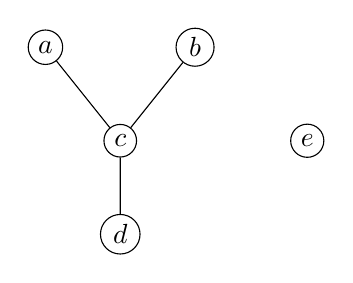
\begin{tikzpicture}[every node/.style={circle,draw,fill=white,inner sep=2pt},scale=.95]
\node (a) at (-1,2.5) {$a$};\node (b) at (1,2.5) {$b$};\node (c) at (0,1.25) {$c$};\node (d) at (0,0) {$d$};\node (e) at (2.5,1.25) {$e$};
\draw (d)--(c)--(a);\draw(c)--(b);
\end{tikzpicture}
\end{minipage}\hfill
\begin{minipage}{.59\linewidth}
\[
M_R=\begin{pmatrix}
1&0&0&0&0\\0&1&0&0&0\\1&1&1&0&0\\1&1&1&1&0\\0&0&0&0&1
\end{pmatrix}.
\]
\end{minipage}
\end{center}
矩阵行列均按 $a,b,c,d,e$ 排列。孤立点仍有自环，所以 $eRe$ 成立。

\subsection{链、反链与有限偏序的分解}
偏序集的子集 $C$ 中任意两元素均可比，则称 $C$ 为\term{链}；子集 $D$ 中任意两个\term{不同}元素均不可比，则称 $D$ 为\term{反链}。单元素集既是链又是反链。本章按课件约定，以元素个数计链长和反链大小；有些书以边数计链长，引用结论时须区分。

反链要求不存在向上可达路径，不能仅凭“没有直接连边”判断。例如 $D_{12}$ 中 $\{1,12\}$ 没有覆盖边，却是链；$\{4,6\}$ 是反链。

\term{有限偏序分解定理：}非空有限偏序集的最长链有 $h$ 个元素，当且仅当把全集划分成反链所需的最少块数为 $h$。

\term{证明：}一条 $h$ 元链与任何反链至多相交于一点，故任何反链划分至少有 $h$ 块。对每个 $x$，定义 $\rho(x)$ 为以 $x$ 为最大元的链的最大元素数。若 $x\prec y$，把 $y$ 接到以 $x$ 结尾的最长链后，得 $\rho(y)\ge\rho(x)+1$。因此相同 $\rho$ 值的元素互不可比，集合 $C_i=\{x\mid\rho(x)=i\}$ 都是反链，$i=1,\ldots,h$。这些非空层构成所需的 $h$ 块划分。

由此，若 $|A|=mn+1$，则至少存在 $n+1$ 元链或 $m+1$ 元反链。否则最长链至多 $n$，可分成至多 $n$ 个反链，每块至多 $m$ 元，从而 $|A|\le mn$，矛盾。此处是二者至少其一，不要求二者同时存在。

\subsection{最大元、最小元、极大元与极小元}
设非空 $B\subseteq A$，$b\in B$。各概念均相对于 $B$ 判断：
\begin{longtable}{p{0.17\linewidth}p{0.76\linewidth}}
\toprule 概念 & 条件\\\midrule\endhead
最大元 & $\forall x\in B\;(x\preceq b)$\\
最小元 & $\forall x\in B\;(b\preceq x)$\\
极大元 & 不存在 $x\in B$ 使 $b\prec x$\\
极小元 & 不存在 $x\in B$ 使 $x\prec b$\\\bottomrule
\end{longtable}
最大元必须支配全部元素，极大元仅要求没有更大的元素，允许有不可比元素。最大元若存在则唯一且为极大元，最小元同理；极大元和极小元可有多个，不同极大元彼此不可比，不同极小元也彼此不可比。

任意非空有限子集均有极大元和极小元：从一点出发，若非极大元，就选择一个更大的点；严格上升不能在有限集合中无限继续，终止处即为极大元。极小元对偶证明。无限集不一定具有极值，例如 $\mathbb Z$ 的通常次序无极大元和极小元。

若非空有限偏序集只有一个极大元，则它是最大元，因为每个元素向上均可延伸到某个极大元。\term{有限性不可省略}：由一个孤立点和一条无上端点的无限链组成的偏序，孤立点是唯一极大元，但不是最大元。

\example{子集中的四种极值（课件例 7.7.8）}
下图的覆盖对为 $(1,2),(1,3),(2,4),(2,5),(3,5),(4,6),(4,7),(5,7),(6,8),(7,8)$。
\begin{center}
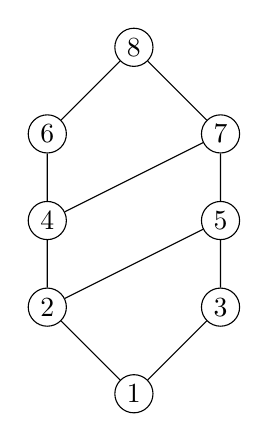
\begin{tikzpicture}[scale=1.1,every node/.style={circle,draw,fill=white,inner sep=2pt}]
\node (a) at (0,0) {$1$};\node (b) at (-1,1) {$2$};\node (c) at (1,1) {$3$};
\node (d) at (-1,2) {$4$};\node (e) at (1,2) {$5$};\node (f) at (-1,3) {$6$};\node (g) at (1,3) {$7$};\node (h) at (0,4) {$8$};
\foreach \u/\v in {a/b,a/c,b/d,b/e,c/e,d/f,d/g,e/g,f/h,g/h}\draw (\u)--(\v);
\end{tikzpicture}
\end{center}
\begin{center}\small
\begin{tabular}{c c c c c}
\toprule $B$ & 最大元 & 最小元 & 极大元集合 & 极小元集合\\\midrule
$\{1,2,3,5\}$ & $5$ & $1$ & $\{5\}$ & $\{1\}$\\
$\{2,3,4,5,6,7\}$ & 无 & 无 & $\{6,7\}$ & $\{2,3\}$\\
$\{4,5,8\}$ & $8$ & 无 & $\{8\}$ & $\{4,5\}$\\
$\{4,5\}$ & 无 & 无 & $\{4,5\}$ & $\{4,5\}$\\\bottomrule
\end{tabular}
\end{center}
虽然全集有最小元 $1$ 和最大元 $8$，子集未必保留它们。判断子集时使用原偏序在子集上的限制，原图中经过子集外元素的路径仍可证明子集内两点可比。

\subsection{上界、下界与上确界、下确界}
在 $\langle A,\preceq\rangle$ 中，对 $B\subseteq A$ 定义
\[
U_A(B)=\{u\in A\mid\forall b\in B\;(b\preceq u)\},\quad
L_A(B)=\{\ell\in A\mid\forall b\in B\;(\ell\preceq b)\}.
\]
其元素分别为 $B$ 的\term{上界}与\term{下界}。它们从整个 $A$ 中寻找，不要求属于 $B$。上界集合的最小元称为\term{上确界}（最小上界）$\sup_A B$；下界集合的最大元称为\term{下确界}（最大下界）$\inf_A B$。

上下界可能有多个，也可能不存在；确界若存在则唯一。仅找到一个极小上界，尚不能断定它是最小上界；它还须小于等于所有上界。$B$ 的最大元若存在，就是 $\sup_A B$；若 $\sup_A B\in B$，它也是 $B$ 的最大元。最小元与下确界对偶。

\example{同一哈斯图中的上下界与确界}
在前例八元素偏序集中：
\begin{center}\small
\begin{tabular}{c c c c c}
\toprule $B$ & $U_A(B)$ & $L_A(B)$ & $\sup_A B$ & $\inf_A B$\\\midrule
$\{2,3,4,5,7\}$ & $\{7,8\}$ & $\{1\}$ & $7$ & $1$\\
$\{2,4,5,6\}$ & $\{8\}$ & $\{1,2\}$ & $8$ & $2$\\
$\{4,5\}$ & $\{7,8\}$ & $\{1,2\}$ & $7$ & $2$\\\bottomrule
\end{tabular}
\end{center}
$\{4,5\}$ 没有最大元和最小元，却同时有上、下确界，且二者都不属于该子集。

在 $D_{12}$ 的整除序中，$B=\{4,6\}$ 的上界集合为 $\{12\}$，下界集合为 $\{1,2\}$，故上确界是 $12$，下确界是 $2$。对于正整数的整除序，有限非空集合的下确界为最大公因数，上确界为最小公倍数；若换成受限的承载集合，则须重新检查候选元素是否属于其中。

\example{孤立点与子集的上下界（课件第 44、64 页）}
设覆盖对为 $(b,d),(b,e),(c,d),(c,e),(d,f),(e,f),(g,h)$，另有孤立点 $a$。图为
\begin{center}
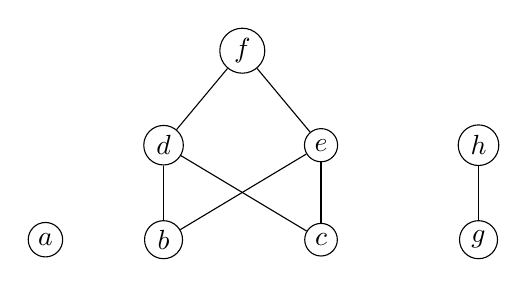
\begin{tikzpicture}[scale=1.0,every node/.style={circle,draw,fill=white,inner sep=2pt}]
\node (a) at (-2.5,0) {$a$};\node (b) at (-1,0) {$b$};\node (c) at (1,0) {$c$};
\node (d) at (-1,1.2) {$d$};\node (e) at (1,1.2) {$e$};\node (f) at (0,2.4) {$f$};
\node (g) at (3,0) {$g$};\node (h) at (3,1.2) {$h$};
\foreach \u/\v in {b/d,b/e,c/d,c/e,d/f,e/f,g/h}\draw (\u)--(\v);
\end{tikzpicture}
\end{center}
关系可恢复为
\[
R=I_A\cup\{(b,d),(b,e),(b,f),(c,d),(c,e),(c,f),(d,f),(e,f),(g,h)\}.
\]
全集的极小元为 $a,b,c,g$，极大元为 $a,f,h$，无最小元和最大元。孤立点 $a$ 同时属于两类极值。对 $B=\{b,c,d\}$，$U_A(B)=\{d,f\}$，上确界是 $d$；下界集合为空，因此没有下确界。

\example{有界而无确界（课件图 7.7.4）}
下图重绘课件的十四元素偏序。覆盖边均由较低点向较高点理解。
\begin{center}
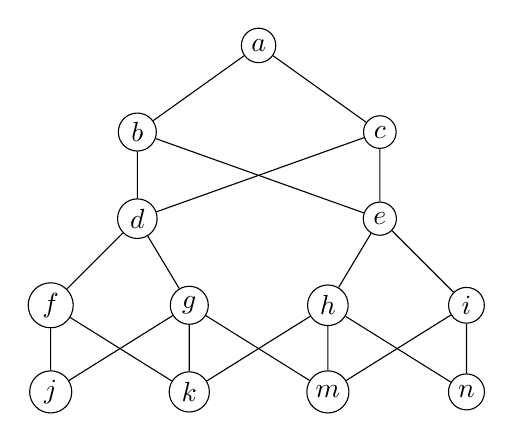
\begin{tikzpicture}[scale=1.1,every node/.style={circle,draw,fill=white,inner sep=2pt}]
\node (a) at (0,4) {$a$};\node (b) at (-1.4,3) {$b$};\node (c) at (1.4,3) {$c$};
\node (d) at (-1.4,2) {$d$};\node (e) at (1.4,2) {$e$};
\node (f) at (-2.4,1) {$f$};\node (g) at (-.8,1) {$g$};\node (h) at (.8,1) {$h$};\node (i) at (2.4,1) {$i$};
\node (j) at (-2.4,0) {$j$};\node (k) at (-.8,0) {$k$};\node (m) at (.8,0) {$m$};\node (n) at (2.4,0) {$n$};
\foreach \u/\v in {b/a,c/a,d/b,d/c,e/b,e/c,f/d,g/d,h/e,i/e,j/f,k/f,j/g,k/g,m/g,k/h,m/h,n/h,m/i,n/i}\draw (\u)--(\v);
\end{tikzpicture}
\end{center}
读图求界时，应分别寻找每个元素的上方可达点或下方可达点，再取交集。对 $B=\{d,e\}$，包括自身的向上可达集合为
\[
\{d,b,c,a\},\qquad\{e,b,c,a\},
\]
其交集为 $U_A(B)=\{a,b,c\}$。同理，两个向下可达集合的交集为 $L_A(B)=\{k,m\}$。其中 $b,c$ 是两个不可比的极小上界，$k,m$ 是两个不可比的极大下界，所以既无上确界也无下确界。

对 $B=\{f,g,h,i\}$，上界仍为 $a,b,c$，不存在下界，因此也无上下确界。图中的 $\{j,k,m,n\}$ 和 $\{f,g,h,i\}$ 都是四元反链；$\{m,h,e,c,a\}$ 是五元链。

\subsection{良序及与全序的关系}
若偏序集的\term{每个非空子集都有最小元}，称它为\term{良序集}（well-ordered set）。这里要求最小元，而非仅有极小元。课件括注中的 well founded relation 通常译为良基关系，应与 well-order 区分。

良序必为全序：对任意 $x,y$，非空子集 $\{x,y\}$ 有最小元，故 $x,y$ 可比。有限全序必为良序：任一非空子集有限，逐个比较即可得到一个不大于其余元素的最小元。因此，在有限偏序中，“全序”和“良序”等价。

无限全序未必良序。正整数通常次序是良序，$\mathbb Z$ 的通常次序不是良序，$(0,1)$ 的通常次序也不是良序，因为集合本身没有最小元。“集合存在某个良序”不表示它当前给定的次序就是良序。一般良序定理在通常的含选择公理集合论中成立，与选择公理等价；不能用它断言实数的通常大小次序为良序。

\subsection{关系构造与包含式的证明}
\example{等价关系的合成仍为原关系（习题课第 5 题）}
设 $R$ 是 $A$ 上的等价关系，$S=\{(a,b)\mid\exists c\in A\;(aRc\land cRb)\}=R\circ R$。传递性给出 $S\subseteq R$；若 $aRb$，取 $c=b$，利用 $bRb$ 得 $aSb$，所以 $R\subseteq S$。故 $S=R$，自然也是等价关系。此结论中传递性负责一个包含方向，自反性负责另一个方向。

\example{两个偏序的直积（习题课第 6 题）}
设 $\langle A,R\rangle,\langle B,S\rangle$ 为偏序集，在 $A\times B$ 上定义
\[
(x,y)T(u,v)\Longleftrightarrow xRu\land ySv.
\]
自反性由 $xRx,ySy$ 得到。若两个有序对相互满足 $T$，则 $xRu,uRx$ 及 $ySv,vSy$，分别由反对称性得 $x=u,y=v$。若 $(x,y)T(u,v)$、$(u,v)T(w,t)$，由 $R,S$ 的传递性得 $xRw,ySt$，即 $(x,y)T(w,t)$。故 $T$ 为偏序。这是逐坐标偏序，不是字典序；即使两个因子均为全序，直积也未必全序，例如通常次序下的 $(1,2)$ 和 $(2,1)$ 不可比。

\example{传递闭包的单调性（习题课第 7 题）}
设 $R\subseteq S$，证明 $t(R)\subseteq t(S)$。由归纳法证明每个 $n\ge1$ 均有 $R^n\subseteq S^n$。初始 $n=1$ 已知；若 $xR^{n+1}y$，则存在 $z$ 使 $xR^nz$ 且 $zRy$。由归纳假设得 $xS^nz$ 且 $zSy$，故 $xS^{n+1}y$。对所有正整数幂取并即得结论。

\exercise
\begin{enumerate}
\item 在 $A=\{1,2,3,4,5,6\}$ 上，设
\[
R=\{1,4\}^2\cup\{2,3,6\}^2\cup\{5\}^2.
\]
判断 $R$ 是否为等价关系，并求商集和有序对数。\\
\term{解：}三块非空、互斥且覆盖 $A$，由划分对应定理可知 $R$ 是等价关系。商集为
\[
A/R=\bigl\{\{1,4\},\{2,3,6\},\{5\}\bigr\}.
\]
有序对数为 $2^2+3^2+1^2=14$。这是课件第 33 页补充题的关系的分块表示。

\item 设 $A=\{1,2,3,4\}$，在 $A\times A$ 上定义 $(x,y)R(u,v)\Longleftrightarrow x+y=u+v$。求所对应的划分。\\
\term{解：}按和 $s=2,\ldots,8$ 分类，得
\begin{align*}
C_2&=\{(1,1)\},&C_3&=\{(1,2),(2,1)\},\\
C_4&=\{(1,3),(2,2),(3,1)\},&C_5&=\{(1,4),(2,3),(3,2),(4,1)\},\\
C_6&=\{(2,4),(3,3),(4,2)\},&C_7&=\{(3,4),(4,3)\},\\
C_8&=\{(4,4)\}.&&
\end{align*}
商集为 $(A\times A)/R=\{C_2,\ldots,C_8\}$，不是 $A/R$。承载集合的元素本身就是有序对。

\item 写出 $\{1,2,3\}$ 的全部划分，并给出相应等价关系。\\
\term{解：}五个划分为
\[
\{\{1\},\{2\},\{3\}\},\quad\{\{1,2\},\{3\}\},\quad
\{\{1,3\},\{2\}\},\quad\{\{2,3\},\{1\}\},\quad\{\{1,2,3\}\}.
\]
对应关系依次为 $I_A$，$I_A\cup\{(1,2),(2,1)\}$，$I_A\cup\{(1,3),(3,1)\}$，$I_A\cup\{(2,3),(3,2)\}$，$A^2$。

\item 设 $R_1,R_2$ 为 $A$ 上的等价关系。判断 $R_1\cap R_2$ 与 $R_1\cup R_2$ 是否一定是等价关系。\\
\term{解：}交集保留自反、对称和传递性，故是等价关系。并集未必传递：在 $\{1,2,3\}$ 上，分别取划分 $\{\{1,2\},\{3\}\}$ 与 $\{\{1\},\{2,3\}\}$ 所对应的关系；并集包含 $(1,2),(2,3)$，却不含 $(1,3)$。

\item 对课件第 68 页的五元素图，覆盖对为 $(e,c),(d,c),(d,b),(c,a),(b,a)$。恢复关系，判定 $aRb,dRa,cRd,cRb,bRe,aRa,eRa$，并求 $B_1=\{c,d,e\}$、$B_2=\{b,c,d\}$、$B_3=\{b,c,d,e\}$ 的上下界和确界。
\begin{center}
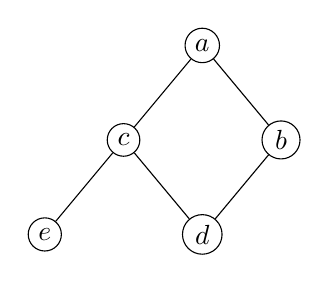
\begin{tikzpicture}[scale=1.0,every node/.style={circle,draw,fill=white,inner sep=2pt}]
\node (a) at (0,2.4) {$a$};\node (b) at (1,1.2) {$b$};\node (c) at (-1,1.2) {$c$};\node (d) at (0,0) {$d$};\node (e) at (-2,0) {$e$};
\foreach \u/\v in {e/c,d/c,d/b,c/a,b/a}\draw (\u)--(\v);
\end{tikzpicture}
\end{center}
\term{解：}关系为
\[
R=I_A\cup\{(e,c),(e,a),(d,c),(d,b),(d,a),(c,a),(b,a)\}.
\]
七个判断依次为假、真、假、假、假、真、真。全集的最大元与唯一极大元为 $a$，极小元为 $d,e$，无最小元。
\begin{center}\small
\begin{tabular}{c c c c c}
\toprule 子集 & 上界 & 下界 & 上确界 & 下确界\\\midrule
$B_1$ & $\{c,a\}$ & $\varnothing$ & $c$ & 无\\
$B_2$ & $\{a\}$ & $\{d\}$ & $a$ & $d$\\
$B_3$ & $\{a\}$ & $\varnothing$ & $a$ & 无\\\bottomrule
\end{tabular}
\end{center}
课件习题课第 4 题的图与本图具有相同的覆盖结构，答案可共用。

\item 在 $A=\{a,b,c,d,e\}$ 上取 $R=I_A\cup\{(c,a),(c,d)\}$，画哈斯图并求极值。\\
\term{解：}仅画 $c$ 向上连接 $a,d$ 的两条边，$b,e$ 为孤立点。极大元为 $a,b,d,e$，极小元为 $b,c,e$，无最大元与最小元。孤立点同时为极大元和极小元。

\item 设 $X$ 是 $n\ge2$ 元有限集，$A=\mathcal P(X)\setminus\{\varnothing,X\}$，按包含关系排序。求极大元、极小元以及最大元、最小元。\\
\term{解：}极小元为所有单元素集；极大元为所有 $X\setminus\{x\}$，$x\in X$。若一个集合至少含两元素，可删去其中一个而仍非空，故非极小；若至少缺两个元素，可增加其中一个而仍不等于 $X$，故非极大。最大元、最小元均不存在。

\item 若一个偏序集有 $13$ 个元素，证明它至少有一条四元链或一条五元反链。\\
\term{解：}$13=4\cdot3+1$，取 $m=4,n=3$，由分解定理的推论立即得到。若所有链均至多三元，可划为至多三个反链，由抽屉原理至少一块含五个元素。
\end{enumerate}

\note{求商集要选择类外的新代表元；反链只比较不同元素；极值从子集内部找，界从整个偏序集中找；有界不保证有确界；哈斯图判序依据向上可达性，不能用数值大小、画图高度或单条覆盖边替代定义。}

\chapterpage{补充：布尔可满足性与建模}
本节保留此前讲义中的 SAT 与数独内容，作为命题逻辑和范式的应用补充，不替代逻辑、集合与关系部分的基本要求。

\subsection{SAT、子句与满足赋值}
\term{布尔可满足性问题}（SAT）是判断给定命题公式是否存在满足赋值，不要求满足赋值唯一。\term{子句}是若干文字的析取，CNF 是子句的合取。3-SAT 常规定每个子句含三个文字，也有教材采用至多三个文字的约定，应说明所用版本。

含 $n$ 个变元的真值表有 $2^n$ 行，完全枚举虽能判定 SAT，但规模随 $n$ 指数增长。DPLL 搜索可结合单位传播；CDCL 方法进一步利用冲突分析与子句学习。计算复杂度高与不可判定不同：SAT 有有限判定方法，一般一阶逻辑可满足性则不存在总能停机的通用判定算法。
\example{单位传播}
CNF 为 $(p\lor q)\land\neg p\land(\neg q\lor r)$。单位子句 $\neg p$ 强制 $p=0$，第一子句因而强制 $q=1$，第三子句强制 $r=1$。得到满足赋值 $011$。单位传播利用已确定的文字逐步简化，而不是直接跳过逻辑约束。

\subsection{数独的 SAT 编码}
对标准 $9\times9$ 数独，设
\[
s_{r,c,d}=1\quad\Longleftrightarrow\quad
\text{第 }r\text{ 行第 }c\text{ 列填数字 }d,
\quad1\le r,c,d\le9.
\]
共 $9^3=729$ 个布尔变量。对任意一组候选文字 $x_1,\ldots,x_k$，“恰好一个为真”可编码为
\[
\operatorname{ExactlyOne}(x_1,\ldots,x_k)
=\left(\bigvee_{i=1}^{k}x_i\right)
\land\bigwedge_{1\le i<j\le k}(\neg x_i\lor\neg x_j).
\]
前半是至少一个，后半是任意一对不能同真。

数独的全部约束为：每格恰好一个数字；每行每个数字恰好一次；每列每个数字恰好一次；每个 $3\times3$ 宫中每个数字恰好一次；已知数字对应变量为真。例如
\begin{align*}
\text{格子 }(r,c):&\quad\operatorname{ExactlyOne}(s_{r,c,1},\ldots,s_{r,c,9}),\\
\text{行 }r\text{ 的数字 }d:&\quad\operatorname{ExactlyOne}(s_{r,1,d},\ldots,s_{r,9,d}),\\
\text{列 }c\text{ 的数字 }d:&\quad\operatorname{ExactlyOne}(s_{1,c,d},\ldots,s_{9,c,d}).
\end{align*}
宫约束对该宫的九个格子应用同一形式。已知 $(r,c)$ 填 $d$，添加单位子句 $s_{r,c,d}$。全部约束合取后为 CNF，满足赋值与数独解对应。

是否存在解和解是否唯一是不同问题。若已有满足赋值，可增加阻断该完整解的子句后再次判断可满足性：若仍可满足，则还有其他解；若不可满足，则原解唯一。这说明形式化建模要同时明确变量、约束与所问性质。

\chapterpage{综合复习、符号与课件索引}
\subsection{逻辑、集合与关系之间的联系}
命题逻辑以真值建立联结词与公式的语义；等值演算把公式化成可比较、可计算的范式；推理理论区分有效性与形式证明。一阶逻辑增加对象、关系和量词，量词演算依赖变量绑定及对象任意性。集合代数则把逻辑条件转成对象的集合关系，并通过容斥进行有限计数。二元关系将对象间的联系表示为有序对集合；等价关系产生划分与商集，偏序关系则通过可比性和覆盖结构研究次序。

逻辑等值、有效推理、集合相等是不同层次的关系：等值保持全部真值；推理只要求前提真时结论真；集合相等要求元素完全一致。它们之间可通过“任取一个对象并判断属于关系”建立联系。

\subsection{关键公式与判定条件}
\begin{enumerate}
\item 蕴涵仅在前真后假时假；$p\to q\equiv\neg p\lor q\equiv\neg q\to\neg p$。
\item 重言式一定可满足；可满足式不一定重言；矛盾式等同不可满足式。
\item 公式层次由嵌套深度确定，二元公式为两子公式层次的最大值加一。
\item 固定变元及顺序后，PDNF 取成真行的 $m_i$，PCNF 取成假行的 $M_i$；两者编号互补，$M_i\equiv\neg m_i$。
\item $n$ 变元有 $2^n$ 种赋值，$2^{2^n}$ 个真值函数；与非、或非各自完备。
\item 推理有效当且仅当前提合取蕴涵结论为重言式；反例要求全部前提真而结论假。
\item 等值式可置换，推理定律通常不可逆；$\vdash$ 与 $\models$ 的定义不同。
\item 一阶解释必须包含非空论域、常项、函数、谓词的解释；开放公式还需自由变量赋值。
\item 否定穿过量词时互换量词；量词跨蕴涵前件时互换，跨后件时不换；移动必须满足自由变量条件。
\item 全称对合取分配，存在对析取分配；另外两个方向一般只能单向推出。
\item 前束化先避免同名变量冲突，再移动量词；不能捕获原自由变量，也不能任意交换混合量词。
\item 全称引入要求对象任意；存在消去使用新见证并解除假设，最终结论不能依赖其名字。
\item $\in$ 是隶属，$\subseteq$ 是包含；$\varnothing$ 与 $\{\varnothing\}$ 不同；$|\mathcal P(A)|=2^{|A|}$ 对有限集成立。
\item $A\subseteq B$ 等价于 $A\cup B=B$、$A\cap B=A$、$A\setminus B=\varnothing$。
\item $A\triangle B=\varnothing$ 当且仅当 $A=B$；差不能任意交换或结合。
\item 容斥交集要用真实重叠数；整除交集取最小公倍数；只会一类与至少一类的计数公式不同。
\item 等价关系要求自反、对称、传递；偏序要求自反、反对称、传递。
\item $aRb\Longleftrightarrow[a]_R=[b]_R$；不同等价类互不相交，$A/R$ 是 $A$ 的划分。
\item $R_1\subseteq R_2$ 当且仅当对应划分满足 $\pi_1\le\pi_2$，关系越小，划分越细。
\item 哈斯图只画覆盖对；恢复有限偏序要加入自环和全部向上可达对。
\item 最大元、最小元属于所考察子集；上下界在整个承载集中寻找；有界不保证有确界。
\item 非空有限偏序有极大、极小元；最长链长度等于最少反链划分块数。
\item 良序要求每个非空子集有最小元；有限时全序与良序等价，无限时一般不等价。
\end{enumerate}

\subsection{常用符号及与课件记法的对应}
\begin{longtable}{p{0.22\linewidth}p{0.71\linewidth}}
\toprule 符号 & 含义与记号说明\\\midrule\endhead
$\neg,\land,\lor$ & 否定、合取、相容析取\\
$\to,\leftrightarrow$ & 公式内部的蕴涵、双条件\\
$\equiv$ & 逻辑等值；课件记作 $\Leftrightarrow$\\
$\models$ & 语义蕴涵；课件重言蕴涵常记作 $\Rightarrow$\\
$\vdash$ & 在指定证明系统中可形式推出\\
$\oplus$ & 命题排斥或；课件也用此符号表示集合对称差\\
$\uparrow,\downarrow$ & 与非、或非\\
$\forall,\exists$ & 全称、存在量词\\
$FV(A)$ & 公式 $A$ 的自由变量集合\\
$A[t/x]$ & 将 $x$ 的自由出现用项 $t$ 合法代替\\
$m_i,M_i$ & 编号 $i$ 的极小项、极大项\\
$\Sigma m,\Pi M$ & 主析取、主合取范式的编号表示\\
$\in,\notin$ & 属于、不属于\\
$\subseteq,\subsetneq$ & 包含、真包含；课件真包含也记作 $\subset$\\
$\cup,\cap,\setminus$ & 并、交、差；课件差记作减号\\
$A^c$ & 相对于固定全集的补；课件记作 $\sim A$\\
$\triangle$ & 集合对称差；课件记作 $\oplus$\\
$\mathcal P(A)$ & 幂集；课件记作 $P(A)$\\
$\bigcup\mathcal A,\bigcap\mathcal A$ & 集合族的广义并、广义交\\
$|A|$ & 集合基数，有限集合时为元素数\\
$A\times B,I_A,E_A$ & 笛卡尔积、恒等关系、全域关系\\
$R^{-1},R\circ S,R^n$ & 逆、合成、关系幂；本章合成为先 $R$ 后 $S$\\
$r(R),s(R),t(R)$ & 自反、对称、传递闭包\\
$[a]_R,A/R$ & 等价类、以不同等价类为元素的商集\\
$\pi_1\le\pi_2$ & 划分细分；不是普通集合族包含\\
$\preceq,\prec$ & 偏序与对应的严格偏序\\
$U_A(B),L_A(B)$ & 相对于承载集 $A$ 的上界、下界集合\\
$\sup_A B,\inf_A B$ & 上确界、下确界\\\bottomrule
\end{longtable}

\subsection{课件覆盖索引}
本讲义以前六章课件和新增的第七章 7.6--7.7 节及其习题课为依据，页数指 PDF 中的页面顺序，包含习题页。行政信息、上课联系方式和仅用于课程导入的材料不作为数学正文。图像习题已按题目含义整理；明显的文字、括号或条件疏漏按数学定义规范表述。
\begin{longtable}{p{0.25\linewidth}p{0.68\linewidth}}
\toprule 课件与页码 & 对应讲义内容\\\midrule\endhead
第一章，4--16 页 & 命题与分类、五种联结词、相容或与排斥或、条件符号化\\
第一章，17--26 页 & 合式公式、层次、赋值、真值表与公式类型\\
第一章，27--34 页 & 第一章例题、练习和类型判定\\
第二章，1--11 页 & 等值式、十六组等值律、置换、等值演算与反例\\
第二章，12--30 页 & 普通范式、极小项与极大项、主范式求法及应用\\
第二章，31--39 页 & 选派建模、真值函数、完备集、与非和或非\\
第二章，40--53 页 & 主范式练习、指定联结词改写、五人选派例题\\
第三章，1--17 页 & 推理形式、有效性判定、推理定律与二难式\\
第三章，18--28 页 & 形式系统、P 系统、直接证明、附加前提与归谬\\
第三章，29--36 页 & 推理反例与构造证明练习\\
第四章，1--10 页 & 个体词、谓词、论域、量词与符号化\\
第四章，11--20 页 & 项、公式、变量出现、闭式、解释、类型、代换实例\\
第四章，21--30 页 & 不同论域解释、量词顺序、成真与成假解释\\
第五章，1--11 页 & 量词等值律、辖域、换名与代替、有限论域展开\\
第五章，12--15 页 & 前束范式及变量冲突处理\\
第五章，16--26 页 & 一阶推理、N 系统、四类量词规则与证明\\
第五章，27--29 页 & 给定解释求值与前束化练习\\
第六章，7--31 页 & 集合概念、表示、隶属、包含、空集、全集、幂集\\
第六章，32--42 页 & 五种运算、文氏图、广义运算与算律\\
第六章，43--55 页 & 包含与恒等式的各类证明方法\\
第六章，56--71 页 & 基数、容斥原理、语言与整除计数、等同规则\\
第六章，72--88 页 & 扫描习题中的层次判断、候选集合、充分必要条件及综合证明\\
第七章 7.6--7.7 文件，1--14 页 & 等价关系、同余、等价类及其基本性质\\
同上，15--33 页 & 商集、划分、一一对应、关系计数、细分\\
同上，34--49 页 & 偏序、全序、覆盖、哈斯图与关系恢复\\
同上，50--62 页 & 链、反链、四类极值、有限分解定理\\
同上，63--73 页 & 上下界、确界、综合图例、良序\\
同上，75--87 页 & 关系运算与闭包、积集分类、偏序直积、包含式证明\\\bottomrule
\end{longtable}
一阶逻辑中自由变量改名按对应赋值理解，避免将其误作固定赋值下的等值；空族广义交明确区分是否固定全集；硬币与着色的计数明确区分对象是否有编号、是否按旋转等同。这些条件用于保证课件中的演算与应用在相应语境下正确。

\subsection{第七章课件的条件与记号修正}
课件第 28 页求商集的选元步骤，应从已求等价类的并集之外选择新代表元；第 50 页反链定义应限定两个不同元素。第 52 页的“没有连线”必须理解为不存在向上可达路径，不能仅检查覆盖边。第 57 页极值的判断不能依赖画图时是否处于同一高度。

第 58 页有限集存在极大元、极小元的结论须补充“非空”；本章给出严格上升链终止的证明，避免第 59 页归纳论证中未检查新元素上方其他元素的缺口。第 60 页分解定理的“至少 $h$ 块”和“恰有 $h$ 块的构造”须同时成立，本章以最长链秩函数给出证明。第 62 页的反链结论来自对反链划分应用抽屉原理，不能理解为每块都含 $m+1$ 个元素。

第 70 页的良序对应 well-order；良基性一般只要求非空子集有极小元，不能与“有最小元”混同。第 73 页良序化定理讨论存在某种次序，不改变给定次序的性质。第 79 页积集分类题的商集承载对象应写成 $(A\times A)/R$。习题课合成运算沿用先左关系、后右关系的约定，避免与其他教材的相反记号混用。

\subsection{综合练习与解答}
\begin{enumerate}
\item 证明 $\Gamma\models C$ 当且仅当 $\bigwedge\Gamma\land\neg C$ 不可满足。\\
\term{解：}若右式可满足，该赋值使全部前提真、结论假，是无效推理的反例。反之，无效推理的反例恰好使该式真。两者取否定即得结论。
\item 已知 $F\equiv\Sigma m(0,2,5,7)$（变元顺序为 $p,q,r$）。求其 PCNF，并用简单公式表示 $F$。\\
\term{解：}PCNF 为 $\Pi M(1,3,4,6)$；四个成真行均满足 $p=r$，$q$ 不影响真值，故 $F\equiv p\leftrightarrow r$。
\item 证明 $\forall x(P(x)\to Q(x)),\forall x(Q(x)\to R(x))\models\forall x(P(x)\to R(x))$。\\
\term{解：}取任意 $u$，全称消去得到两个蕴涵，假言三段论得 $P(u)\to R(u)$；因 $u$ 不受前提限制，全称引入得结论。
\item 将 $\neg\exists x(P(x)\land\forall yR(x,y))$ 化为前束范式。\\
\term{解：}$\forall x(\neg P(x)\lor\exists y\neg R(x,y))\equiv\forall x\exists y(\neg P(x)\lor\neg R(x,y))$。
\item 证明 $A\subseteq B$ 当且仅当 $A\cap B^c=\varnothing$，并用一阶逻辑写出它。\\
\term{解：}$A\cap B^c=A\setminus B$，使用包含的等价条件即可。逻辑形式为 $\forall x(x\in A\to x\in B)\Longleftrightarrow\neg\exists x(x\in A\land x\notin B)$。
\item 求 $1$ 至 $100$ 中至少被 $2,3,5$ 中一个整除的数目，以及三者都不能整除的数目。\\
\term{解：}至少一个为 $50+33+20-16-10-6+3=74$；均不能整除者为 $100-74=26$。
\end{enumerate}
\end{document}
